% Options for packages loaded elsewhere
\PassOptionsToPackage{unicode}{hyperref}
\PassOptionsToPackage{hyphens}{url}
%
\documentclass[
]{book}
\usepackage{amsmath,amssymb}
\usepackage{lmodern}
\usepackage{ifxetex,ifluatex}
\ifnum 0\ifxetex 1\fi\ifluatex 1\fi=0 % if pdftex
  \usepackage[T1]{fontenc}
  \usepackage[utf8]{inputenc}
  \usepackage{textcomp} % provide euro and other symbols
\else % if luatex or xetex
  \usepackage{unicode-math}
  \defaultfontfeatures{Scale=MatchLowercase}
  \defaultfontfeatures[\rmfamily]{Ligatures=TeX,Scale=1}
\fi
% Use upquote if available, for straight quotes in verbatim environments
\IfFileExists{upquote.sty}{\usepackage{upquote}}{}
\IfFileExists{microtype.sty}{% use microtype if available
  \usepackage[]{microtype}
  \UseMicrotypeSet[protrusion]{basicmath} % disable protrusion for tt fonts
}{}
\makeatletter
\@ifundefined{KOMAClassName}{% if non-KOMA class
  \IfFileExists{parskip.sty}{%
    \usepackage{parskip}
  }{% else
    \setlength{\parindent}{0pt}
    \setlength{\parskip}{6pt plus 2pt minus 1pt}}
}{% if KOMA class
  \KOMAoptions{parskip=half}}
\makeatother
\usepackage{xcolor}
\IfFileExists{xurl.sty}{\usepackage{xurl}}{} % add URL line breaks if available
\IfFileExists{bookmark.sty}{\usepackage{bookmark}}{\usepackage{hyperref}}
\hypersetup{
  pdftitle={Notes on and Solutions for Statistical Rethinking},
  pdfauthor={Alexander Pastukhov},
  hidelinks,
  pdfcreator={LaTeX via pandoc}}
\urlstyle{same} % disable monospaced font for URLs
\usepackage{color}
\usepackage{fancyvrb}
\newcommand{\VerbBar}{|}
\newcommand{\VERB}{\Verb[commandchars=\\\{\}]}
\DefineVerbatimEnvironment{Highlighting}{Verbatim}{commandchars=\\\{\}}
% Add ',fontsize=\small' for more characters per line
\usepackage{framed}
\definecolor{shadecolor}{RGB}{248,248,248}
\newenvironment{Shaded}{\begin{snugshade}}{\end{snugshade}}
\newcommand{\AlertTok}[1]{\textcolor[rgb]{0.94,0.16,0.16}{#1}}
\newcommand{\AnnotationTok}[1]{\textcolor[rgb]{0.56,0.35,0.01}{\textbf{\textit{#1}}}}
\newcommand{\AttributeTok}[1]{\textcolor[rgb]{0.77,0.63,0.00}{#1}}
\newcommand{\BaseNTok}[1]{\textcolor[rgb]{0.00,0.00,0.81}{#1}}
\newcommand{\BuiltInTok}[1]{#1}
\newcommand{\CharTok}[1]{\textcolor[rgb]{0.31,0.60,0.02}{#1}}
\newcommand{\CommentTok}[1]{\textcolor[rgb]{0.56,0.35,0.01}{\textit{#1}}}
\newcommand{\CommentVarTok}[1]{\textcolor[rgb]{0.56,0.35,0.01}{\textbf{\textit{#1}}}}
\newcommand{\ConstantTok}[1]{\textcolor[rgb]{0.00,0.00,0.00}{#1}}
\newcommand{\ControlFlowTok}[1]{\textcolor[rgb]{0.13,0.29,0.53}{\textbf{#1}}}
\newcommand{\DataTypeTok}[1]{\textcolor[rgb]{0.13,0.29,0.53}{#1}}
\newcommand{\DecValTok}[1]{\textcolor[rgb]{0.00,0.00,0.81}{#1}}
\newcommand{\DocumentationTok}[1]{\textcolor[rgb]{0.56,0.35,0.01}{\textbf{\textit{#1}}}}
\newcommand{\ErrorTok}[1]{\textcolor[rgb]{0.64,0.00,0.00}{\textbf{#1}}}
\newcommand{\ExtensionTok}[1]{#1}
\newcommand{\FloatTok}[1]{\textcolor[rgb]{0.00,0.00,0.81}{#1}}
\newcommand{\FunctionTok}[1]{\textcolor[rgb]{0.00,0.00,0.00}{#1}}
\newcommand{\ImportTok}[1]{#1}
\newcommand{\InformationTok}[1]{\textcolor[rgb]{0.56,0.35,0.01}{\textbf{\textit{#1}}}}
\newcommand{\KeywordTok}[1]{\textcolor[rgb]{0.13,0.29,0.53}{\textbf{#1}}}
\newcommand{\NormalTok}[1]{#1}
\newcommand{\OperatorTok}[1]{\textcolor[rgb]{0.81,0.36,0.00}{\textbf{#1}}}
\newcommand{\OtherTok}[1]{\textcolor[rgb]{0.56,0.35,0.01}{#1}}
\newcommand{\PreprocessorTok}[1]{\textcolor[rgb]{0.56,0.35,0.01}{\textit{#1}}}
\newcommand{\RegionMarkerTok}[1]{#1}
\newcommand{\SpecialCharTok}[1]{\textcolor[rgb]{0.00,0.00,0.00}{#1}}
\newcommand{\SpecialStringTok}[1]{\textcolor[rgb]{0.31,0.60,0.02}{#1}}
\newcommand{\StringTok}[1]{\textcolor[rgb]{0.31,0.60,0.02}{#1}}
\newcommand{\VariableTok}[1]{\textcolor[rgb]{0.00,0.00,0.00}{#1}}
\newcommand{\VerbatimStringTok}[1]{\textcolor[rgb]{0.31,0.60,0.02}{#1}}
\newcommand{\WarningTok}[1]{\textcolor[rgb]{0.56,0.35,0.01}{\textbf{\textit{#1}}}}
\usepackage{longtable,booktabs,array}
\usepackage{calc} % for calculating minipage widths
% Correct order of tables after \paragraph or \subparagraph
\usepackage{etoolbox}
\makeatletter
\patchcmd\longtable{\par}{\if@noskipsec\mbox{}\fi\par}{}{}
\makeatother
% Allow footnotes in longtable head/foot
\IfFileExists{footnotehyper.sty}{\usepackage{footnotehyper}}{\usepackage{footnote}}
\makesavenoteenv{longtable}
\usepackage{graphicx}
\makeatletter
\def\maxwidth{\ifdim\Gin@nat@width>\linewidth\linewidth\else\Gin@nat@width\fi}
\def\maxheight{\ifdim\Gin@nat@height>\textheight\textheight\else\Gin@nat@height\fi}
\makeatother
% Scale images if necessary, so that they will not overflow the page
% margins by default, and it is still possible to overwrite the defaults
% using explicit options in \includegraphics[width, height, ...]{}
\setkeys{Gin}{width=\maxwidth,height=\maxheight,keepaspectratio}
% Set default figure placement to htbp
\makeatletter
\def\fps@figure{htbp}
\makeatother
\setlength{\emergencystretch}{3em} % prevent overfull lines
\providecommand{\tightlist}{%
  \setlength{\itemsep}{0pt}\setlength{\parskip}{0pt}}
\setcounter{secnumdepth}{5}
\usepackage{booktabs}
\ifluatex
  \usepackage{selnolig}  % disable illegal ligatures
\fi
\usepackage[]{natbib}
\bibliographystyle{apalike}

\title{Notes on and Solutions for Statistical Rethinking}
\author{Alexander Pastukhov}
\date{2021-04-14}

\begin{document}
\maketitle

{
\setcounter{tocdepth}{1}
\tableofcontents
}
\hypertarget{precis}{%
\chapter{Precis}\label{precis}}

This is a collection of notes that attempt to provide further details and intuition for some topics, such as loss functions, information theory, information criteria, MCMC algorithms, etc. This material is \textbf{free to use} and is licensed under the \href{https://creativecommons.org/licenses/by-nc-nd/4.0/}{Creative Commons Attribution-NonCommercial-NoDerivatives V4.0 International License}.

\hypertarget{loss-functions}{%
\chapter{Loss functions}\label{loss-functions}}

The purpose of this comment is to give you an intuition about loss functions, mentioned in chapter 3. In particular, I want you to understand why different loss functions (L0, L1, and L2) correspond to different point-estimates (mode, median, and mean). Plus, I want you to understand that you can view a choice of a likelihood function, as in picking Gaussian in chapter 4, as being analogous to picking a loss function.

I am afraid that the easiest way to explain why an \emph{L2} loss results in \emph{mean} is via a derivative. So, if you are not confident in your basic calculus skill, it might be useful for you to first watch a few episodes of \href{https://www.youtube.com/playlist?list=PLZHQObOWTQDMsr9K-rj53DwVRMYO3t5Yr}{Essense of Calculus} series by Grant Sanderson, a.k.a. \href{https://www.3blue1brown.com/}{3Blue1Brown}. I would suggest watching at least the first three episodes (actually, I would recommend to watch the whole series) but if you are short on time watch only episode 2\footnote{Although, if you skip episode 1, you won't know why it is \emph{obvious} that area of a circle is \(\pi\cdot r^2\)}.

\hypertarget{loss-function-the-concept}{%
\section{Loss function, the concept}\label{loss-function-the-concept}}

Imagine that you are selling ice-cream on a beach, so we can assume it is a narrow strip of sand and, therefore, a one-dimensional problem. It is hot, so \emph{everyone} wants ice-cream (obviously) and you want to maximize the number of ice-creams you sell (obviously). People are distributed in some random (not necessarily uniform or symmetric) way along the beach, so the question is: Where do you put your \emph{single} ice-cream stand to maximize your profits? The answer depends on your choice of the \emph{loss function} that describes how distance between a particular person and your stand influences whether person will buy your ice-cream. In other words, it describes the \emph{cost} of getting to your stand, i.e.~walking all-the-way through the sand in that heat. This \emph{cost} clearly depends on the distance and in the simplest case, it is linearly proportional to the distance: If you need to walk twice the distance, your costs for getting an ice-cream are twice as high. However, the relationship between the distance and cost does not have to be so simple and linear and this is why we have many different \emph{loss} / \emph{cost} functions.

We can write a loss/cost function more formally as \(L(stand, person_i)\) where \texttt{stand} is the location of your stand and \texttt{person\_i} is a location of a particular ith person. The cost can be either zero or positive, i.e., we assume there is no benefit in walking all the way, only no or some cost. So, where should you put your ice-cream stand?

\begin{center}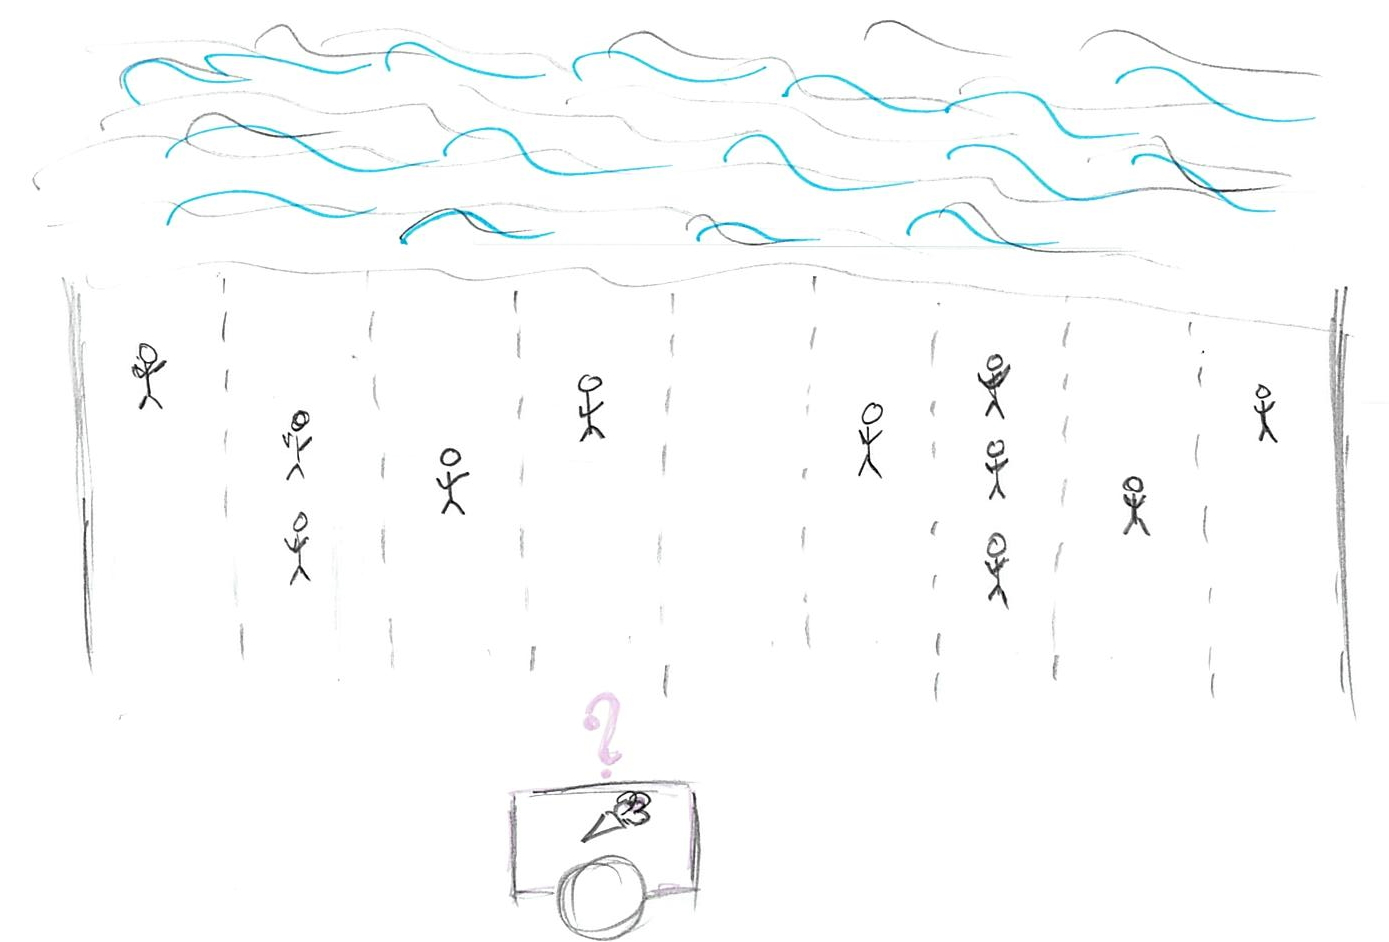
\includegraphics[width=1\linewidth]{images/loss-functions-where-to} \end{center}

\hypertarget{l0-mode}{%
\section{L0 (mode)}\label{l0-mode}}

The simplest loss function is\\
\[L0(stand, person_i) =  \begin{cases}
0, stand == person_i \\
\infty, stand \neq person_i
\end{cases}\]

This function assumes that everybody hates walking so much, that \emph{any} walk is unbearable and should be avoided. Thus, there is no cost for getting your ice-cream only for people who are positioned right next to your stand. For everybody else, even one meter away, the costs of walking are infinite, so they won't bother and, therefore, won't buy your ice-cream. Still, we are in the business of selling one, so where do we put our stand given how lazy our customers are? Well, we just find the biggest group of people and put our stand next to them. No one else will come but at least you got the biggest group of customers you could. If you look at the \emph{distribution} of your customers along the beach this is the highest peak (that you peak) and it is called the \emph{mode} of the distribution.

\begin{center}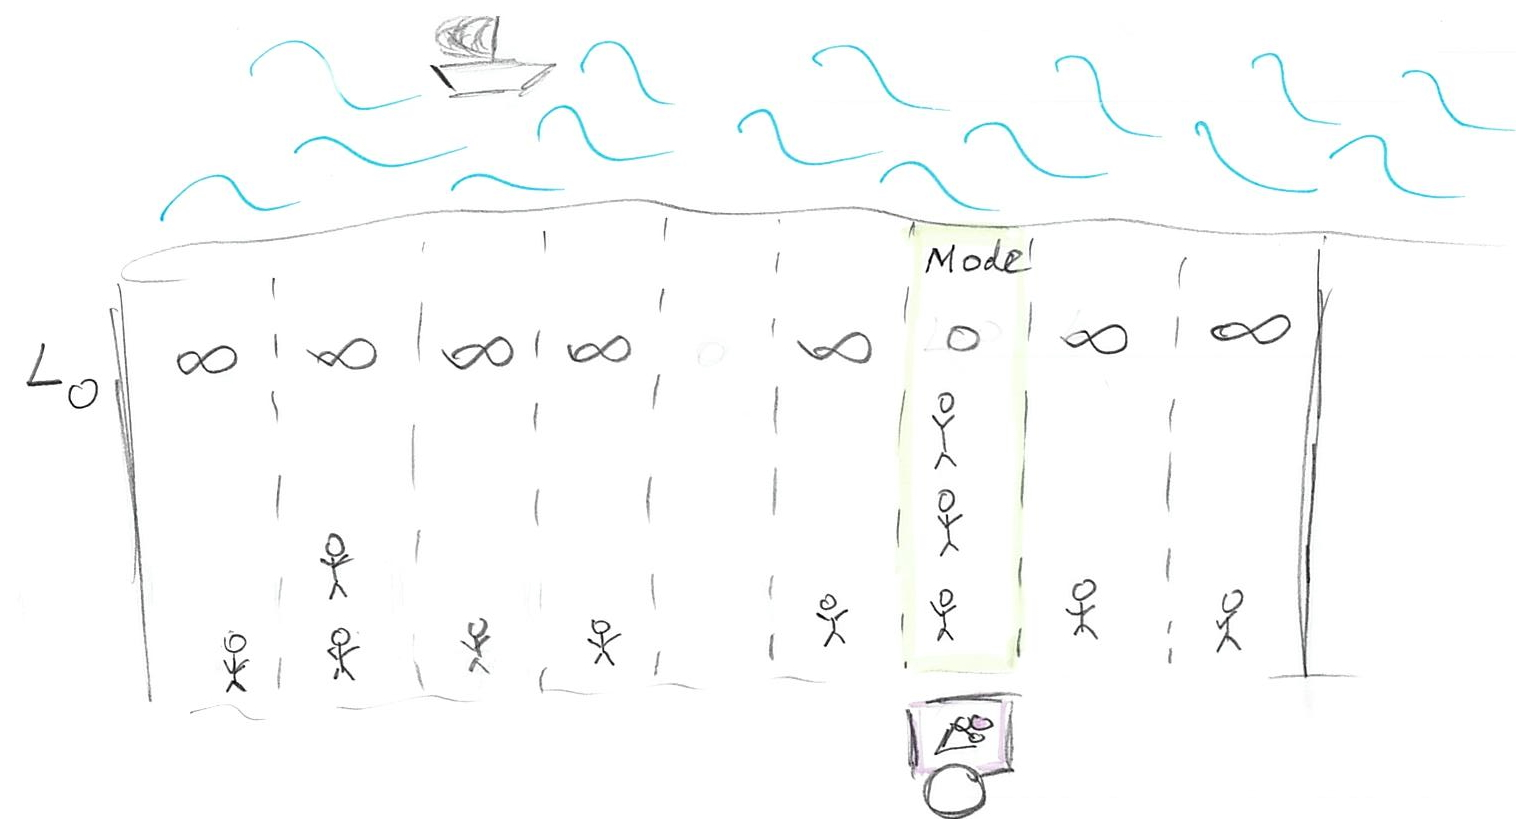
\includegraphics[width=1\linewidth]{images/loss-functions-L0} \end{center}

\hypertarget{l1-median}{%
\section{L1 (median)}\label{l1-median}}

The next loss function, that I already mentioned, assumes a simple linear relationship between the distance and the cost
\[L1(stand, person_i) = |person_i - stand|\]
In other words, the cost is equal to distance (we need \texttt{\textbar{}\ \textbar{}} to get an absolute value, because the person could be ``to the left of'' of stand, in which case \texttt{person\ -\ stand} distance will be negative). So, where should we put our stand? Let us start at a fairly random location so that 3 of our customers are on the left and 7 are on the right.

\begin{center}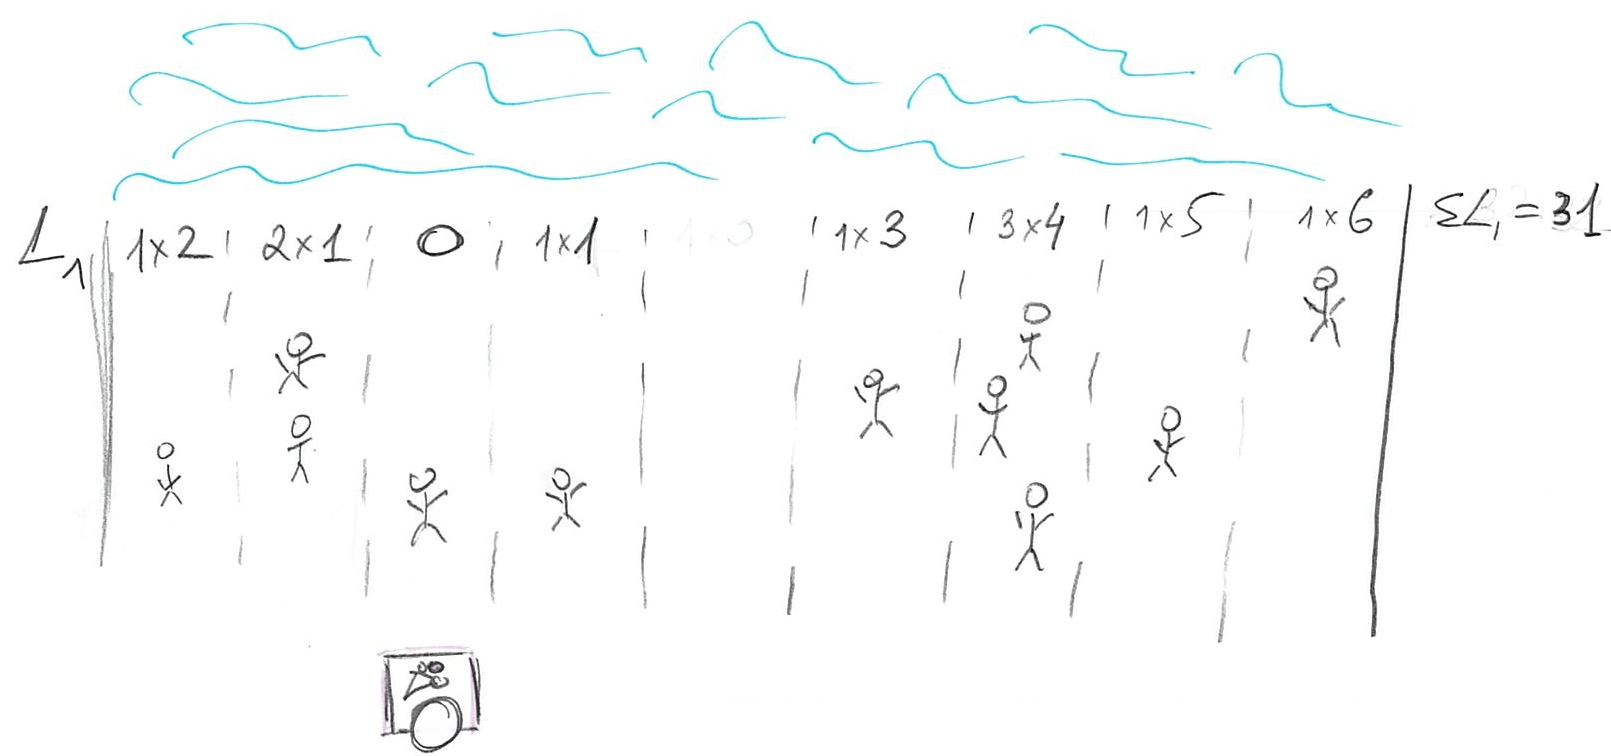
\includegraphics[width=1\linewidth]{images/loss-functions-L1-off-median} \end{center}

We can, in principle, compute the actual cost but it is simpler to ask the question of whether we can \emph{improve} on that cost by moving somewhere else? Imagine that we move to the left where \emph{minority} of our customers are. Now we have 1 on the left and 8 on the right (plus 2 more at our location).

\begin{center}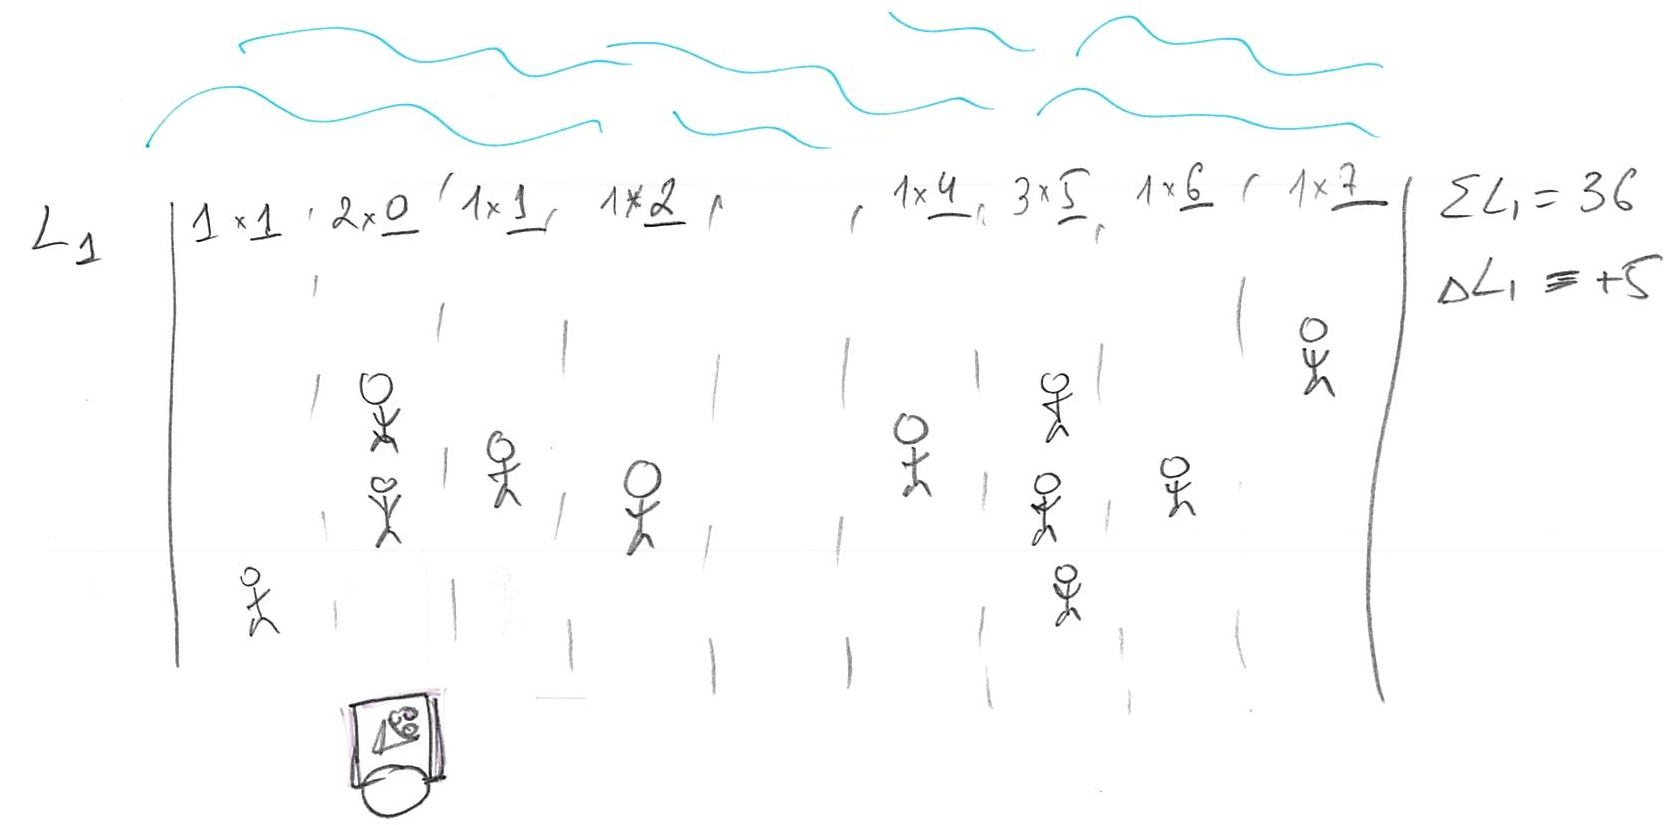
\includegraphics[width=1\linewidth]{images/loss-functions-L1-left} \end{center}

The problem is, we moved \emph{away} from the majority of the people so our total cost is \emph{original cost - 3 (improvement due to moving close to minority) + 8 (increase in loss due to moving away from majority)}, so \(\Delta L1 = +5\). Oops, we made it worse! How about moving to the \emph{right}?

\begin{center}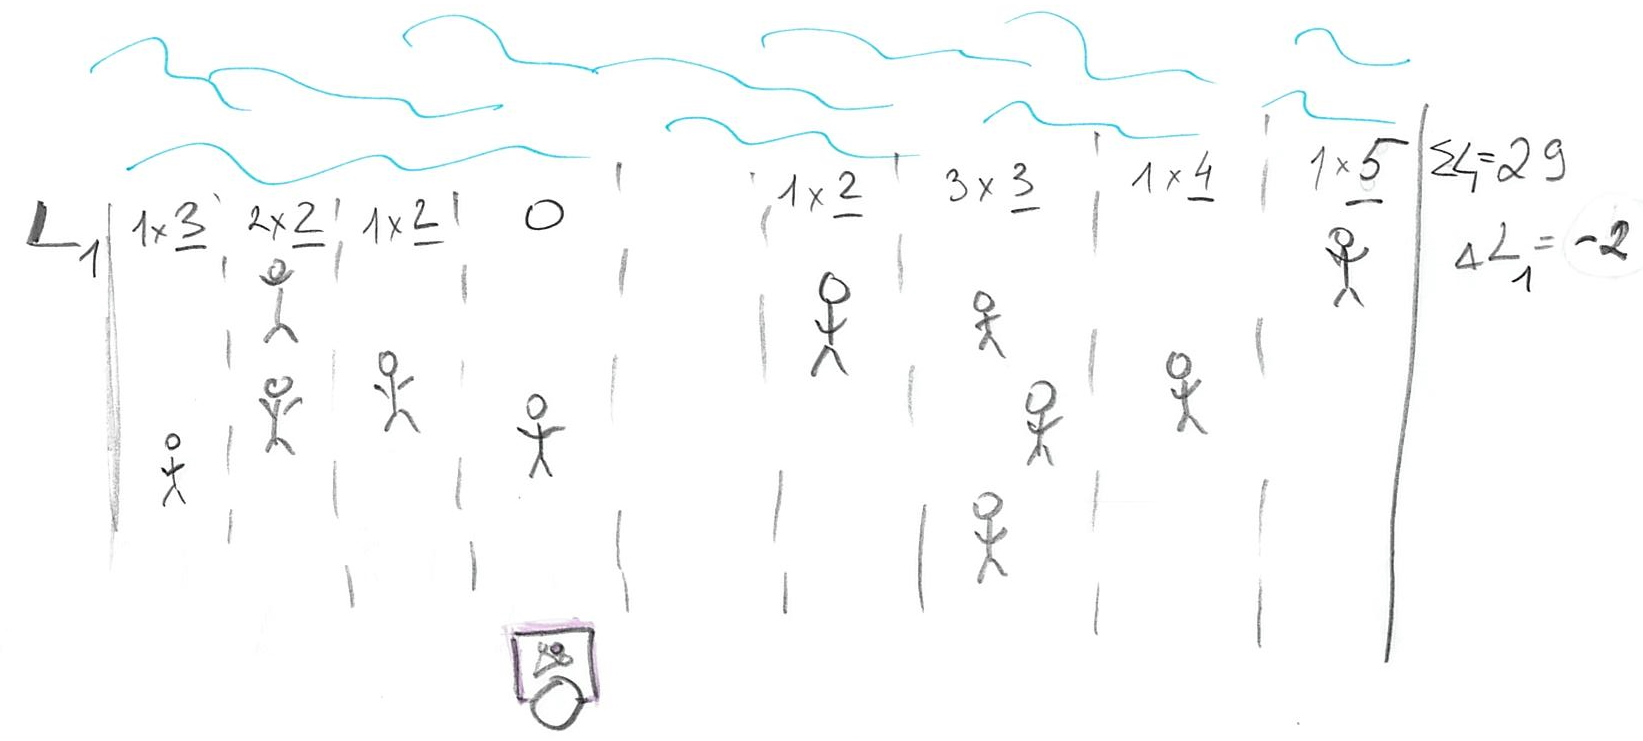
\includegraphics[width=1\linewidth]{images/loss-functions-L1-right} \end{center}

Now that we move \emph{towards} the majority of customers, we have four on the left and six on the right (plus one at our location). The change in cost is \emph{original cost + 4 (loss due to moving away from minority) - 6 (improvement due to moving towards majority)}, so \(\Delta L1 = -2\). Which gives us an idea: we should try to get even closer to that majority by keeping walking to the right! Eventually, you will get to point of the 50/50. Should you keep moving to the right? Should you move to the left? Should you move at all?

\begin{center}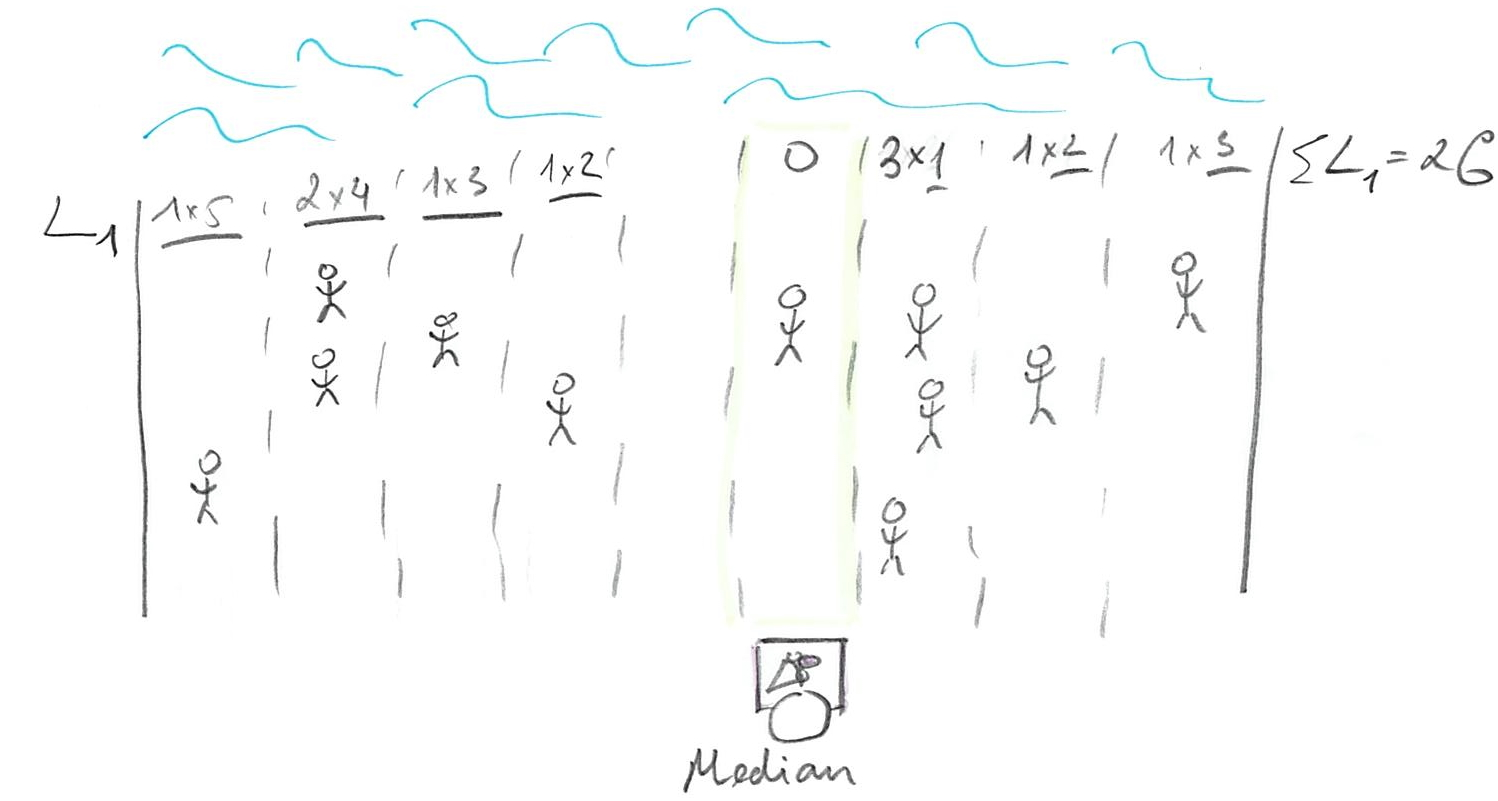
\includegraphics[width=1\linewidth]{images/loss-functions-L1-median} \end{center}

There is no point in moving to the left. You just came from where because moving to the right made things better. However, if you keep moving to the right, you will keep passing people, so that majority now will be on the left and you would be walking \emph{away} from the majority, raising the costs (and your losses). So, once you get to point where half of your customers are on the left and half are on the right, you cannot do any better. Any movement that gets you from 50/50 means there are more customers on one side (say left, if you moved to the right) and, as we already figured out, your best strategy is to move towards the majority, which gets you back where you started at 50/50 point. That 50/50 points split, when half of customers / probability mass is on one side and half is on the other, is called \emph{median}.

\hypertarget{l2-mean}{%
\section{L2 (mean)}\label{l2-mean}}

The classic loss function is Euclidean distance \[L2(stand, person_i) = (person - stand)^2\]
Here, every next step becomes progressively harder for our customers. The cost of walking 1 meter is 1 (unit of effort). But walking 2 is \(2^2 = 4\) and is \(3^2=9\) for 3 meters. Thus, the penalty (cost/loss) for being further away from your stand increases as a power law. Still, one needs to sell ice-cream, so one needs to find the best spot where total cost is minimal

\[L2(stand, person) = \sum_{i=1}^{N}{(person_i - stand)^2}\]

\begin{center}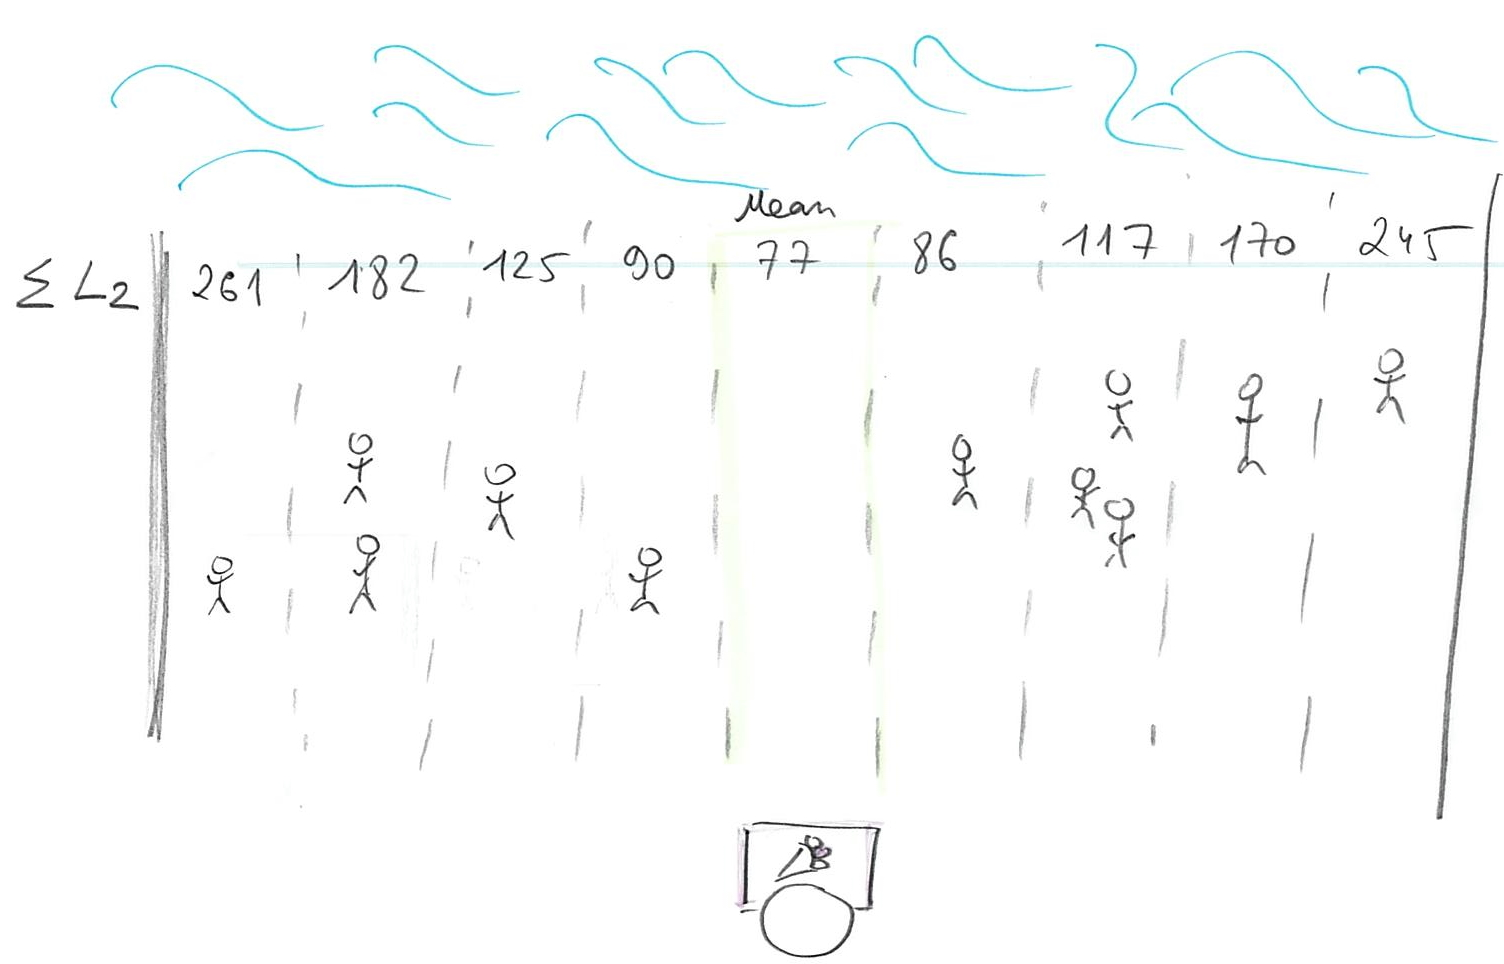
\includegraphics[width=1\linewidth]{images/loss-functions-L2-mean} \end{center}

Or, we can compute the minimal \emph{average} cost by dividing the sum by the total number of customers \texttt{N}:
\[<L2(stand, person)> = \frac{1}{N}\sum_{i=1}^{N}{(person_i - stand)^2}\]

Conceptually, you find that minimum by walking along the beach in the direction that reduces the cost until you hit the point where it start going up again. This strategy is called \emph{gradient descent} and, generally speaking, this is how computer finds minima computationally: They make steps in different directions to see which way is down and keep going until things start going up. However, in one-dimensional well-behaving case we have here things are even simpler as you can use calculus to figure out the solution analytically. If you watched the videos I advertised above, you'll know that the \emph{derivative} of the function is zero at the extrema (minima or maxima), so we just need to differentiate our average \emph{L2} over position of the stand and find where it is zero\footnote{I've nicked the derivations from {[}\url{https://stats.stackexchange.com/a/312997}{]}}.

\[\frac{\partial L2}{\partial stand} = -\frac{2}{N}\sum_{i=1}^{N}{(person_i - stand)}\]
As we want
\[\frac{\partial L2}{\partial stand} = 0\]
we state
\[\frac{2}{N}\sum_{i=1}^{N}{(person_i - stand)} = 0.\]

Opening up brackets and rearranging we get

\[- \frac{2}{N}\sum_{i=1}^{N}{person_i} + \frac{2 \cdot N}{N} \cdot stand = 0 \\
2 \cdot stand = \frac{2}{N}\sum_{i=1}^{N}{person_i} \\
stand = \frac{1}{N}\sum_{i=1}^{N}{person_i}\]

So, the optimal location of your stand is the \emph{mean}: an average location of all people on the beach.

\hypertarget{l1-median-vs.-l2-mean}{%
\section{L1 (median) vs.~L2 (mean)}\label{l1-median-vs.-l2-mean}}

One problem about the \emph{mean} is that it is sensitive to outliers. Because the costs grow as a power law, this approach favors a lot of medium-sized distances over lots of smalls ones plus one really large one. Thus, a single person at a far side of the beach would have a big influence on your stand's location (you already saw the difference in the example above). In data analysis, this means that those outliers will pull your estimates away from the majority of responses. Which is why it might be a good idea to consider using \texttt{median} rather than \texttt{mean}. If you distribution is symmetric, the difference will be negligible but in presence of outliers \texttt{median}, as a point-estimate, is more robust.

\hypertarget{choosing-a-likelihood}{%
\section{Choosing a likelihood}\label{choosing-a-likelihood}}

So far we talked about selling ice-cream on the beach but same question of choosing your loss function applies when you are trying to fit a distribution or a regression line, as in chapter 4. Here, you also have a point-estimate (regression line at each point) and you try to put it in such a way as to minimize the costs of having data points off that line (the distance from the point-estimate of the line and each data point is called a \emph{residual}). The classic way is to use \emph{L2} distance and the approach is called \emph{ordinary least squares}, as you try to minimize squared residuals.

Alternatively, you can express same costs-of-being-off-the-line using a distribution, such as Gaussian. You put its peak (mean) at the (candidate) location of your point estimate (that point has highest probability, so lowest cost) and the loss is computed as a probability of the residual (distance-to-the-point). You can think about it in terms of the probability that a person will go and buy ice-cream from your stand.

\begin{center}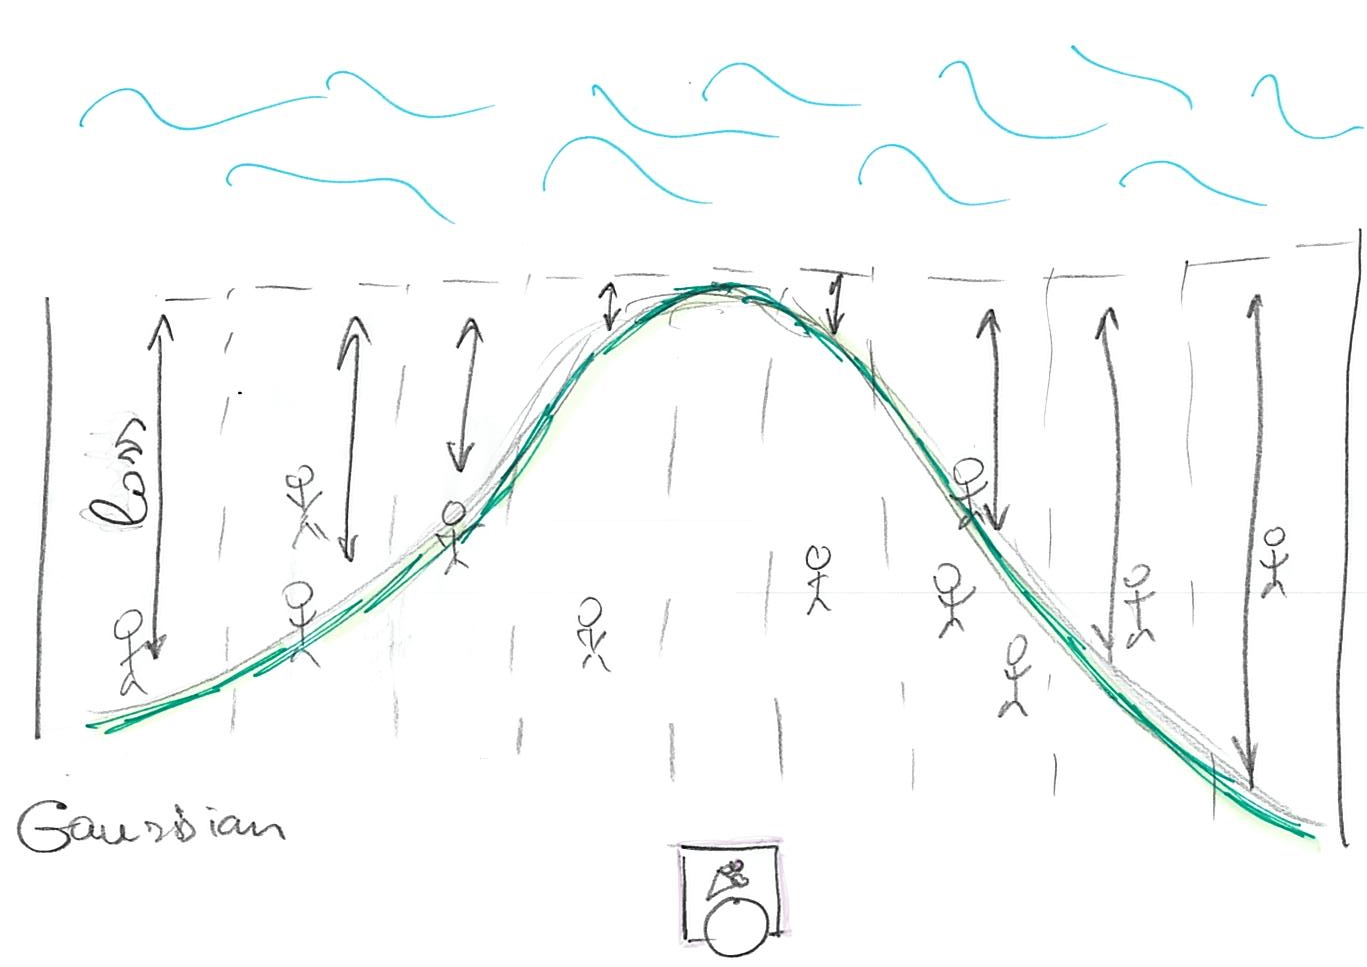
\includegraphics[width=1\linewidth]{images/loss-functions-Gaussian} \end{center}

The Gaussian is special because it uses L2 distance, see \((x - \mu)^2\) inside the exponential:
\[f(x) = \frac{1}{\sigma \sqrt(2 \pi)}e^{\left(-\frac{1}{2}\frac{(x - \mu)^2}{\sigma^2}\right)}\]

so using it is equivalent to fitting via ordinary least squares. However, as McElreath hinted, you can choose different priors that are different not only in the distance-to-loss formula (like \emph{L1} is different from \emph{L2}) but also in symmetry. Both \emph{L1} and \emph{L2} (and Gaussian) ignore the sign of the distance. It does not matter whether customers are on the left or on the right. Other distributions, such as Beta, Gamma, or Log Normal are not symmetric, so the same distance will cost differently depending on the side the customer is at.

\begin{center}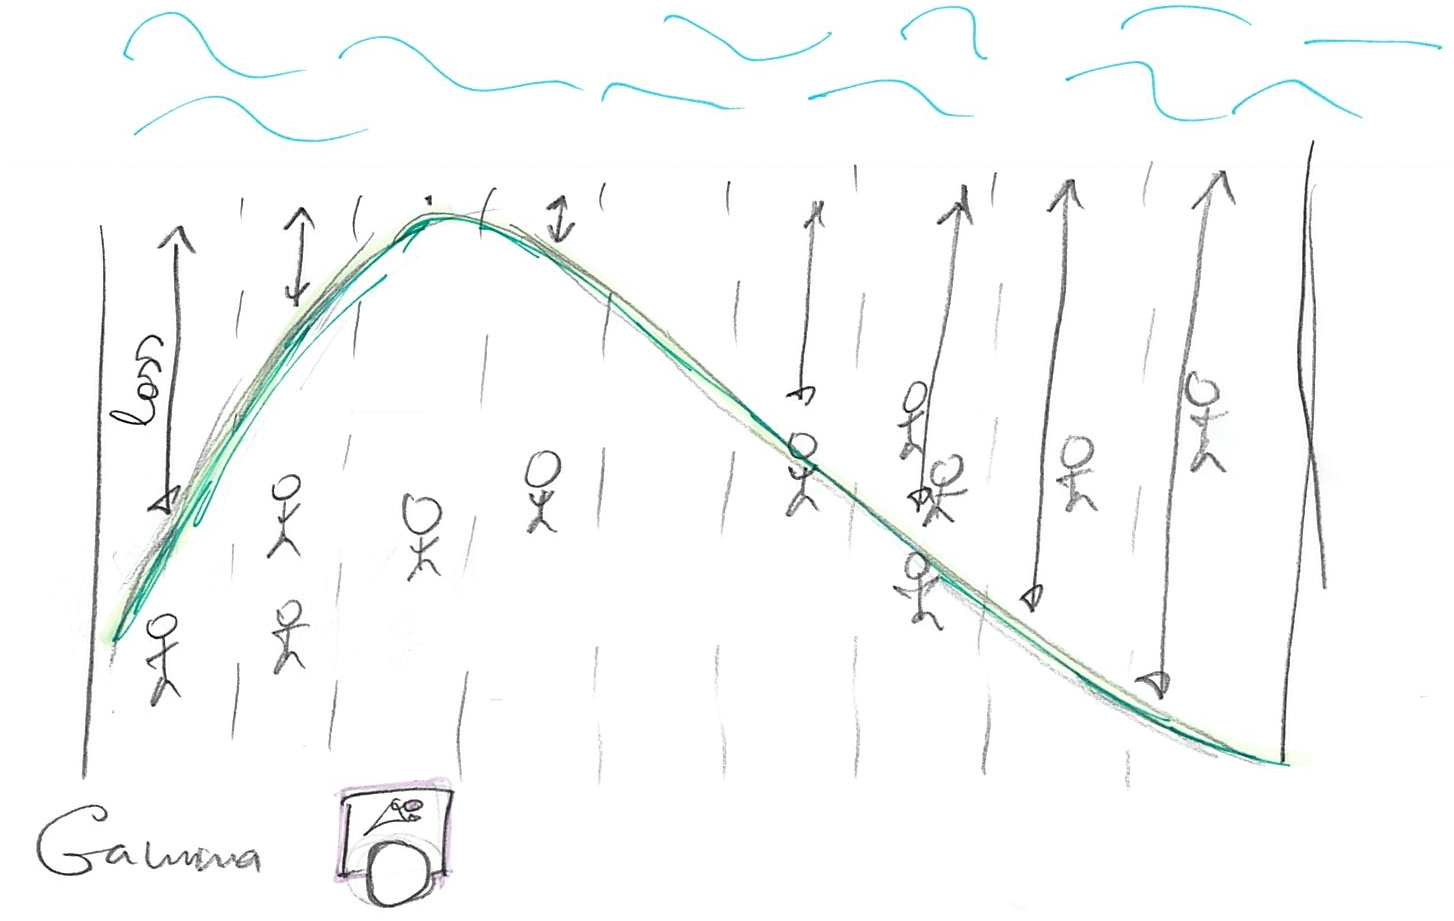
\includegraphics[width=1\linewidth]{images/loss-functions-Gamma} \end{center}

This allows you to think about the choice of your likelihood distribution in terms of choosing a loss function. Both describe how tolerant you are for points to be off the point estimate (regression line). For example, a t-distribution has heavier tails than a Gaussian (if you want to sound like a real mathematician, you say ``leptokurtic''), so its losses for outliers (penalty for larger residuals) are lower. Using it instead of a Gaussian would be similar to changing the loss function from L2 to be more like L1 (e.g.~\(|person_i - stand|^{1.5}\)). Conversely, you can pick a symmetric distribution that is narrower than a Gaussian to make residuals penalty even higher (e.g.~using \((person_i - stand)^{4}\)). You can also consider other properties: Should it be symmetric? Should it operate only within certain range (1..7 for a Likert scale, 0..1 for proportions, positive values for Gamma)? Should it weight all points equally? As you saw in the examples above, picking a different function moves your cart (regression line), so you should keep in mind that using a different likelihood will move the regression line and produce different estimates and predictions.

How do you pick a likelihood/loss function? It depends on the kind of data you have, on your knowledge about the process that generated the data, robustness of inferences in the presence of outliers, etc. However, most real-life cases you are likely to encounter will be covered by the distributions described in the book (Gaussian, exponential, binomial, Poisson, Gamma, etc.). After finishing the book, you will have a basic understanding of which are most appropiate in typical cases. The atypical cases you'll have to research yourself!

\hypertarget{gaussian-in-frenquentist-versus-bayesian-statistics}{%
\section{Gaussian in frenquentist versus Bayesian statistics}\label{gaussian-in-frenquentist-versus-bayesian-statistics}}

Later on in the book McElreath will note that erroneously assuming normal distribution for residuals ruins your inferences in frequentist statistics but not in Bayesian. This is because picking a distribution means different things in frequentist and Bayesian. As I wrote above, in the Bayesian case, likelihood is merely a loss function that translate distance from a data point to a regression line (residual) into a penalty (again, it determines just how tolerant you are for points off the line). Thus, you are using penalties for \emph{observed residuals} and having a bad loss function will make your posterior distribution suboptimal but you still can make inferences because it still is based on your actual residuals.

In contrast, in frequentist statistics, when you are stating that your observed residuals are a sample from a particular distribution, your actual residuals are used to determine parameters of this distribution. Then, however, you make your inferences using \emph{that distribution} not the residuals themselves. This is a very strong conjecture and probably the biggest leap of faith in frequentist statistics saying ``I know the true distribution''. Problem is, if you got your likelihood function / distribution wrong, your inferences are based on a model that describes \emph{something else} not your data. For example, you have a proportion data but you assume Gaussian distribution for residuals and build a model as if your residuals are always symmetrically distributed (not squashed on one side by floor or celing). That model will not be about your data, it will be about normally distributed \emph{something else}. The numbers for that \emph{something else} may look good (or bad) but they are not the numbers you are interested in. This is a mistake that is remarkably easy to do because computers won't stop you from making it. Think back to Chapter 1: Golems don't care! You can abuse any statistical model/test and they will simply spit out the numbers, even if tests are completely unsuitable for your data. Making sure that distribution is correct and that you are doing the right thing is on you, not the Golem!

\hypertarget{directed-acyclic-graphs-and-causal-reasoning}{%
\chapter{Directed Acyclic Graphs and Causal Reasoning}\label{directed-acyclic-graphs-and-causal-reasoning}}

\hypertarget{peering-into-a-black-box}{%
\section{Peering into a black box}\label{peering-into-a-black-box}}

To better understand the relationship between data and statistical analysis on the one hand and DAGs (directed acyclic graphs) on the other hand, I came up with an electric engineering metaphor\footnote{Dear electric engineers, yes, I know that's not quite how it works but it is still a good metaphor!}. Imagine that you have an electric device that you cannot take apart. However, there are certain points where you can connect your multimeter and check whether current flows between these two points. You also have a schematics for the device but you have no idea whether it is accurate. The names of the connector nodes match but \emph{the connectivity} between them is anybody's guess. So, what do you do? You look at the schematics and identify two nodes where current should \emph{definitely flow} and you measure whether that is the case. Do you have signal? Good, that means that \emph{at least with respect to the connectivity between these two nodes} you schematics is not completely wrong. No signal? Sorry, your schematics is no good, find a different one or try making one yourself. Conversely, you can identify two nodes, so that \emph{no current} should flow between them and measure it \emph{empirically}. No current? Good! Current? Bad, your schematics is wrong.

The relationship between the device and the schematics is that of the large (device) and small (schematics) world. Your job is to iteratively adjust the latter, so that it matches the former. You need to keep prodding the black box until predictions from your schematics start matching the actual readings. Only then you can say that you understand how device works and you can make predictions about what it will do under different conditions. Although testing based on schematics can be automated, generating such schematics is a creating process. It depends on our knowledge about devices of that kind and about individual exposed nodes.

Hopefully, you can see how it maps on our observational or experimental data (large world, readings from the device) and DAGs (small world, presumed schematics). As a scientist, you \emph{guess}\footnote{If you feel that science is not about guessing, you are wrong and I have Richard Feynman on my side! You always start by guessing a particular law or rule and then use empirical data to check whether your guess was correct. If you made an \emph{educated} guess, your chances of it being correct are higher, so your job is to study the field and prior work to make your guess as educated as possible. But, at the end, it is still a guess and it can be wrong. Good news, at least in my experience, is that guesses that turn out to be spectacularly wrong are the most informative ones, as they reveal something unexpected and, thus, hitherto unknown about the process.} the causal relationships between individual variables and you draw a schematics for that (a DAG). Using this DAG, you identify pairs of variables that must be dependent or independent \emph{assuming your DAG is correct} and check the data on whether this is indeed the case. It is? Good, your DAG is not (entirely) wrong! They are not? Bad news, their causal relationship is different from what you (or others in prior work) came up with. You need to modify DAG or draw a completely different one, just like a engineer must modify the schematics.

Note that this process is the opposite to that in a typical multivariate analysis approach using, say, ANOVA. In the latter case, you throw \emph{everything} together, including some/all interactions between the terms, and try figuring out causal relationship between individual independent and the dependent variable based on magnitude and significance of individual terms. So, \emph{first} you run the statistical analysis and \emph{then} you make your inferences about causal relationships. In causal reasoning using DAG, you \emph{first} formulate causal relationships and \emph{then} you use statistical analysis to check whether these relationship are correct. The second approach is much more powerful, because you can run ANOVA only once but you can formulate many DAGs that describe your data and test them iteratively, refining your understanding step-by-step. Moreover, ANOVA (or any other regression model like that) is about identifying relationships between invididual independent and the signle dependent variable (individual coefficients tell you how independent variables can be used to predict the dependent). DAG-based analysis allows you to predict and test relationship between pairs of \emph{dependent} variables as well, decomposing your complex model into \emph{testable} and \emph{verifyable} chunks. It is a more involved and time-consuming approach but it gives you much deeper understanding of the process you are styding compared to ``throw everything into ANOVA and hope it will magically figure it out''.

Moreover, causal calculus via DAGs has another trick up its sleeve. You can use \emph{conditional probabilities} (see below) to flip the relationship between variables. If two variables are independent, they may be dependent when conditioned on some third variable. Or vice versa, depedent variables can become \emph{conditionally independent}. This means that your predictions about connectivity between pairs of variables can be both more specific (e.g., they are related via a third variable or they both independently cause that third variable) and more testable, as you now have two \emph{opposite} predictions for the same pair of variables! You can check that current flows when it should (unconditional probability) and \emph{does not flow} once you condition it on the third variable. Both tests match? DAG is not that bad! One or none match? Back to the drawing board!

\hypertarget{turning-unconditional-dependence-into-conditional-independence}{%
\section{Turning unconditional dependence into conditional independence}\label{turning-unconditional-dependence-into-conditional-independence}}

Below, you will see how multiple regression can show conditional independence of two variable in case of the fork DAG in divorce data. However, there is another more general way to understand this concept it terms of conditional probabilities \(Pr(M|A)\) and \(Pr(D|A)\). For this, it helps to understand condition probabilities as \emph{filtering} operation. When we compute conditional probability for a \emph{specific} value of \(A\), this means that we slice the data, keeping only whose values of \(M\) and \(D\) that correspond to that chosen level of \(A\). It is easier to understand, if we visualize that conditional-probability-as-filtering in synthetic data. For illustration purposes, I will synthesize divorce data, keeping the relationships but I will space marriage age linearly and generate the data so that there are 20 data points for each age (makes it easier to see and understand).

\begin{Shaded}
\begin{Highlighting}[]
\FunctionTok{set.seed}\NormalTok{(}\DecValTok{84321169}\NormalTok{)}
\NormalTok{N }\OtherTok{\textless{}{-}} \DecValTok{180}
\NormalTok{sigma\_noise }\OtherTok{\textless{}{-}} \FloatTok{0.5}
\CommentTok{\# we repeat each value of age 10 times to make filtering operation easier to see}
\NormalTok{sim\_waffles }\OtherTok{\textless{}{-}} \FunctionTok{tibble}\NormalTok{(}\AttributeTok{MedianAgeMarriage =} \FunctionTok{rep}\NormalTok{(}\FunctionTok{seq}\NormalTok{(}\SpecialCharTok{{-}}\DecValTok{2}\NormalTok{, }\DecValTok{2}\NormalTok{, }\AttributeTok{length.out=}\DecValTok{9}\NormalTok{), }\DecValTok{20}\NormalTok{), }
                      \AttributeTok{Divorce =} \FunctionTok{rnorm}\NormalTok{(N, MedianAgeMarriage, sigma\_noise),}
                      \AttributeTok{Marriage =} \SpecialCharTok{{-}}\FunctionTok{rnorm}\NormalTok{(N, MedianAgeMarriage, sigma\_noise))}

\NormalTok{MD\_plot }\OtherTok{\textless{}{-}} 
  \FunctionTok{ggplot}\NormalTok{(}\AttributeTok{data=}\NormalTok{sim\_waffles, }\FunctionTok{aes}\NormalTok{(}\AttributeTok{x=}\NormalTok{Marriage, }\AttributeTok{y=}\NormalTok{Divorce)) }\SpecialCharTok{+} 
    \FunctionTok{geom\_smooth}\NormalTok{(}\AttributeTok{method=}\StringTok{"lm"}\NormalTok{, }\AttributeTok{formula=}\NormalTok{y}\SpecialCharTok{\textasciitilde{}}\NormalTok{x) }\SpecialCharTok{+} 
    \FunctionTok{geom\_point}\NormalTok{() }\SpecialCharTok{+} 
    \FunctionTok{xlab}\NormalTok{(}\StringTok{"Marriage rate"}\NormalTok{) }\SpecialCharTok{+} 
    \FunctionTok{ylab}\NormalTok{(}\StringTok{"Divorce rate"}\NormalTok{)}
  
\NormalTok{AD\_plot }\OtherTok{\textless{}{-}} 
  \FunctionTok{ggplot}\NormalTok{(}\AttributeTok{data=}\NormalTok{sim\_waffles, }\FunctionTok{aes}\NormalTok{(}\AttributeTok{x=}\NormalTok{MedianAgeMarriage, }\AttributeTok{y=}\NormalTok{Divorce)) }\SpecialCharTok{+} 
    \FunctionTok{geom\_smooth}\NormalTok{(}\AttributeTok{method=}\StringTok{"lm"}\NormalTok{, }\AttributeTok{formula=}\NormalTok{y}\SpecialCharTok{\textasciitilde{}}\NormalTok{x) }\SpecialCharTok{+} 
    \FunctionTok{geom\_point}\NormalTok{() }\SpecialCharTok{+} 
    \FunctionTok{xlab}\NormalTok{(}\StringTok{"Median age marriage"}\NormalTok{) }\SpecialCharTok{+} 
    \FunctionTok{ylab}\NormalTok{(}\StringTok{"Divorce rate"}\NormalTok{)}
  
\NormalTok{AM\_plot }\OtherTok{\textless{}{-}} 
  \FunctionTok{ggplot}\NormalTok{(}\AttributeTok{data=}\NormalTok{sim\_waffles, }\FunctionTok{aes}\NormalTok{(}\AttributeTok{x=}\NormalTok{MedianAgeMarriage, }\AttributeTok{y=}\NormalTok{Marriage)) }\SpecialCharTok{+} 
    \FunctionTok{geom\_smooth}\NormalTok{(}\AttributeTok{method=}\StringTok{"lm"}\NormalTok{, }\AttributeTok{formula=}\NormalTok{y}\SpecialCharTok{\textasciitilde{}}\NormalTok{x) }\SpecialCharTok{+} 
    \FunctionTok{geom\_point}\NormalTok{() }\SpecialCharTok{+} 
    \FunctionTok{xlab}\NormalTok{(}\StringTok{"Median age marriage"}\NormalTok{) }\SpecialCharTok{+} 
    \FunctionTok{ylab}\NormalTok{(}\StringTok{"Marriage rate"}\NormalTok{)}

\NormalTok{MD\_plot }\SpecialCharTok{|}\NormalTok{ AD\_plot }\SpecialCharTok{|}\NormalTok{ AM\_plot}
\end{Highlighting}
\end{Shaded}

\begin{center}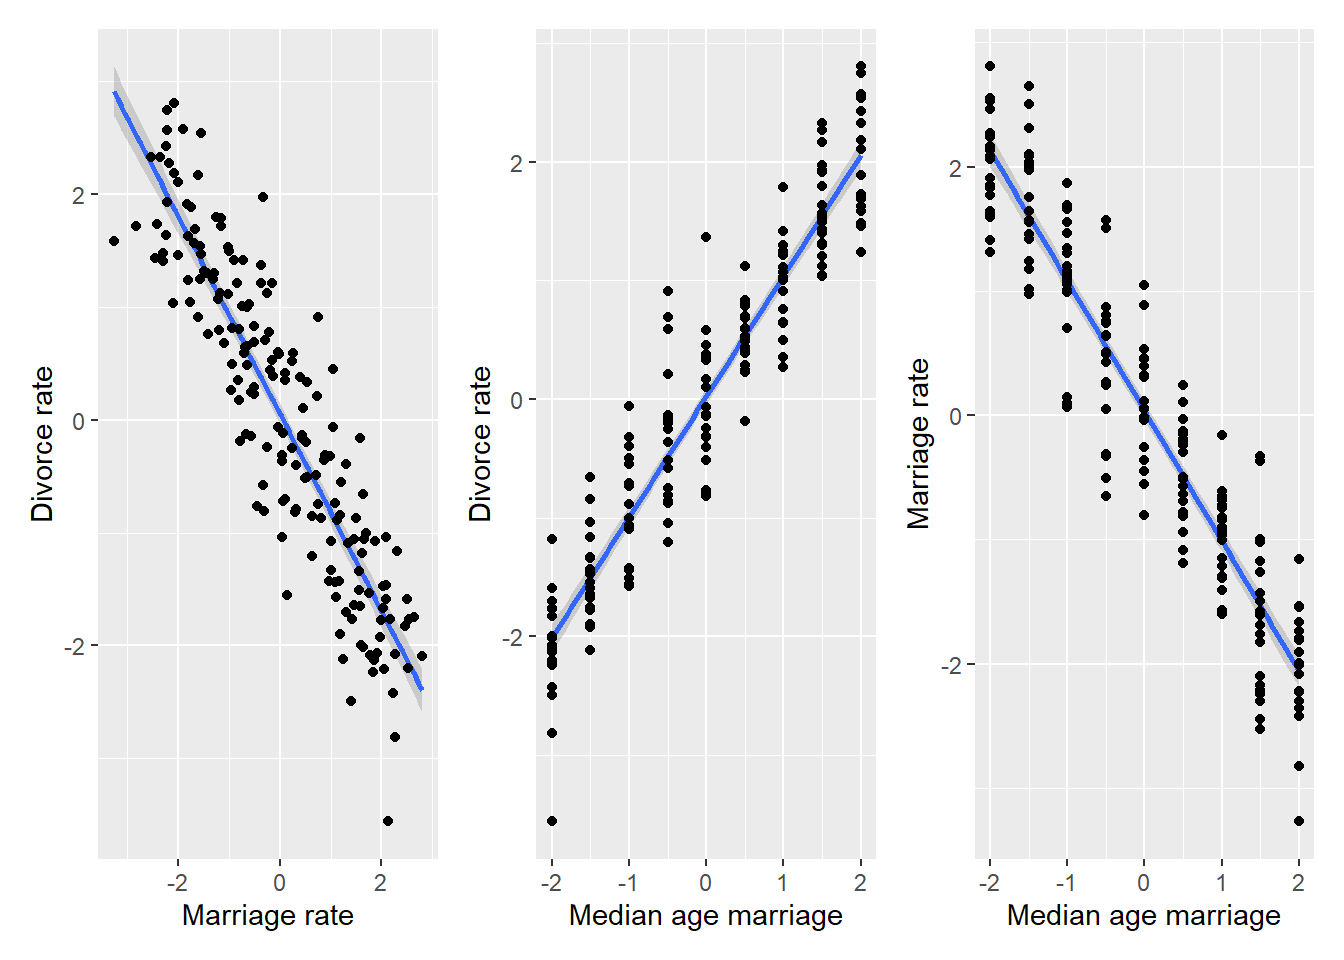
\includegraphics[width=1\linewidth]{notes-on-statistical-rethinking_files/figure-latex/unnamed-chunk-11-1} \end{center}

As you can see, all variables being dependent on each other, as in case of the original data. However, let us pick an arbitrary value, say \(A=1\)\footnote{The data is ``standardized'', therefore, age of 1 is one standard deviation away from the mean marriage rate.} and see which dots on the left plot will be selected via \emph{filtering} on that value.

\begin{Shaded}
\begin{Highlighting}[]
\NormalTok{MD\_plot }\OtherTok{\textless{}{-}} 
  \FunctionTok{ggplot}\NormalTok{(}\AttributeTok{data=}\NormalTok{sim\_waffles, }\FunctionTok{aes}\NormalTok{(}\AttributeTok{x=}\NormalTok{Marriage, }\AttributeTok{y=}\NormalTok{Divorce)) }\SpecialCharTok{+} 
    \FunctionTok{geom\_smooth}\NormalTok{(}\AttributeTok{method=}\StringTok{"lm"}\NormalTok{, }\AttributeTok{formula=}\NormalTok{y}\SpecialCharTok{\textasciitilde{}}\NormalTok{x, }\AttributeTok{alpha=}\FloatTok{0.1}\NormalTok{) }\SpecialCharTok{+} 
    \FunctionTok{geom\_point}\NormalTok{(}\AttributeTok{data=}\NormalTok{sim\_waffles }\SpecialCharTok{\%\textgreater{}\%} \FunctionTok{filter}\NormalTok{(MedianAgeMarriage }\SpecialCharTok{==} \DecValTok{1}\NormalTok{), }\AttributeTok{color=}\StringTok{"red"}\NormalTok{) }\SpecialCharTok{+}
    \FunctionTok{geom\_point}\NormalTok{(}\AttributeTok{data=}\NormalTok{sim\_waffles }\SpecialCharTok{\%\textgreater{}\%} \FunctionTok{filter}\NormalTok{(MedianAgeMarriage }\SpecialCharTok{!=} \DecValTok{1}\NormalTok{), }\AttributeTok{alpha=}\FloatTok{0.15}\NormalTok{) }\SpecialCharTok{+} 
    \FunctionTok{xlab}\NormalTok{(}\StringTok{"Marriage rate"}\NormalTok{) }\SpecialCharTok{+} 
    \FunctionTok{ylab}\NormalTok{(}\StringTok{"Divorce rate"}\NormalTok{) }
\NormalTok{AD\_plot }\OtherTok{\textless{}{-}} 
  \FunctionTok{ggplot}\NormalTok{(}\AttributeTok{data=}\NormalTok{sim\_waffles, }\FunctionTok{aes}\NormalTok{(}\AttributeTok{x=}\NormalTok{MedianAgeMarriage, }\AttributeTok{y=}\NormalTok{Divorce)) }\SpecialCharTok{+} 
    \FunctionTok{geom\_smooth}\NormalTok{(}\AttributeTok{method=}\StringTok{"lm"}\NormalTok{, }\AttributeTok{formula=}\NormalTok{y}\SpecialCharTok{\textasciitilde{}}\NormalTok{x) }\SpecialCharTok{+} 
    \FunctionTok{geom\_point}\NormalTok{(}\AttributeTok{data=}\NormalTok{sim\_waffles }\SpecialCharTok{\%\textgreater{}\%} \FunctionTok{filter}\NormalTok{(MedianAgeMarriage }\SpecialCharTok{==} \DecValTok{1}\NormalTok{), }\AttributeTok{color=}\StringTok{"red"}\NormalTok{) }\SpecialCharTok{+}
    \FunctionTok{geom\_point}\NormalTok{(}\AttributeTok{data=}\NormalTok{sim\_waffles }\SpecialCharTok{\%\textgreater{}\%} \FunctionTok{filter}\NormalTok{(MedianAgeMarriage }\SpecialCharTok{!=} \DecValTok{1}\NormalTok{), }\AttributeTok{alpha=}\FloatTok{0.15}\NormalTok{) }\SpecialCharTok{+} 
    \FunctionTok{xlab}\NormalTok{(}\StringTok{"Median age marriage"}\NormalTok{) }\SpecialCharTok{+} 
    \FunctionTok{ylab}\NormalTok{(}\StringTok{"Divorce rate"}\NormalTok{)}
  
\NormalTok{AM\_plot }\OtherTok{\textless{}{-}}
  \FunctionTok{ggplot}\NormalTok{(}\AttributeTok{data=}\NormalTok{sim\_waffles, }\FunctionTok{aes}\NormalTok{(}\AttributeTok{x=}\NormalTok{Marriage, }\AttributeTok{y=}\NormalTok{MedianAgeMarriage)) }\SpecialCharTok{+} 
    \FunctionTok{geom\_smooth}\NormalTok{(}\AttributeTok{method=}\StringTok{"lm"}\NormalTok{, }\AttributeTok{formula=}\NormalTok{y}\SpecialCharTok{\textasciitilde{}}\NormalTok{x) }\SpecialCharTok{+} 
    \FunctionTok{geom\_point}\NormalTok{(}\AttributeTok{data=}\NormalTok{sim\_waffles }\SpecialCharTok{\%\textgreater{}\%} \FunctionTok{filter}\NormalTok{(MedianAgeMarriage }\SpecialCharTok{==} \DecValTok{1}\NormalTok{), }\AttributeTok{color=}\StringTok{"red"}\NormalTok{) }\SpecialCharTok{+}
    \FunctionTok{geom\_point}\NormalTok{(}\AttributeTok{data=}\NormalTok{sim\_waffles }\SpecialCharTok{\%\textgreater{}\%} \FunctionTok{filter}\NormalTok{(MedianAgeMarriage }\SpecialCharTok{!=} \DecValTok{1}\NormalTok{), }\AttributeTok{alpha=}\FloatTok{0.15}\NormalTok{) }\SpecialCharTok{+} 
    \FunctionTok{ylab}\NormalTok{(}\StringTok{"Median age marriage"}\NormalTok{) }\SpecialCharTok{+} 
    \FunctionTok{xlab}\NormalTok{(}\StringTok{"Marriage rate"}\NormalTok{) }

\NormalTok{MD\_A1\_plot }\OtherTok{\textless{}{-}} 
  \FunctionTok{ggplot}\NormalTok{(}\AttributeTok{data=}\NormalTok{sim\_waffles }\SpecialCharTok{\%\textgreater{}\%} \FunctionTok{filter}\NormalTok{(MedianAgeMarriage }\SpecialCharTok{==} \DecValTok{1}\NormalTok{), }
         \FunctionTok{aes}\NormalTok{(}\AttributeTok{x=}\NormalTok{Marriage, }\AttributeTok{y=}\NormalTok{Divorce)) }\SpecialCharTok{+} 
    \FunctionTok{geom\_smooth}\NormalTok{(}\AttributeTok{method=}\StringTok{"lm"}\NormalTok{, }\AttributeTok{formula=}\NormalTok{y}\SpecialCharTok{\textasciitilde{}}\NormalTok{x, }\AttributeTok{color=}\StringTok{"red"}\NormalTok{) }\SpecialCharTok{+} 
    \FunctionTok{geom\_point}\NormalTok{(}\AttributeTok{color=}\StringTok{"red"}\NormalTok{) }\SpecialCharTok{+}
    \FunctionTok{xlab}\NormalTok{(}\StringTok{"Marriage rate"}\NormalTok{) }\SpecialCharTok{+} 
    \FunctionTok{ylab}\NormalTok{(}\StringTok{"Divorce rate"}\NormalTok{) }\SpecialCharTok{+}
    \FunctionTok{labs}\NormalTok{(}\AttributeTok{subtitle =} \StringTok{"Pr( |Mariage Age = 1)"}\NormalTok{)}

\NormalTok{(AD\_plot }\SpecialCharTok{|}\NormalTok{ MD\_plot) }\SpecialCharTok{/}
\NormalTok{(MD\_A1\_plot }\SpecialCharTok{|}\NormalTok{AM\_plot)}
\end{Highlighting}
\end{Shaded}

\begin{center}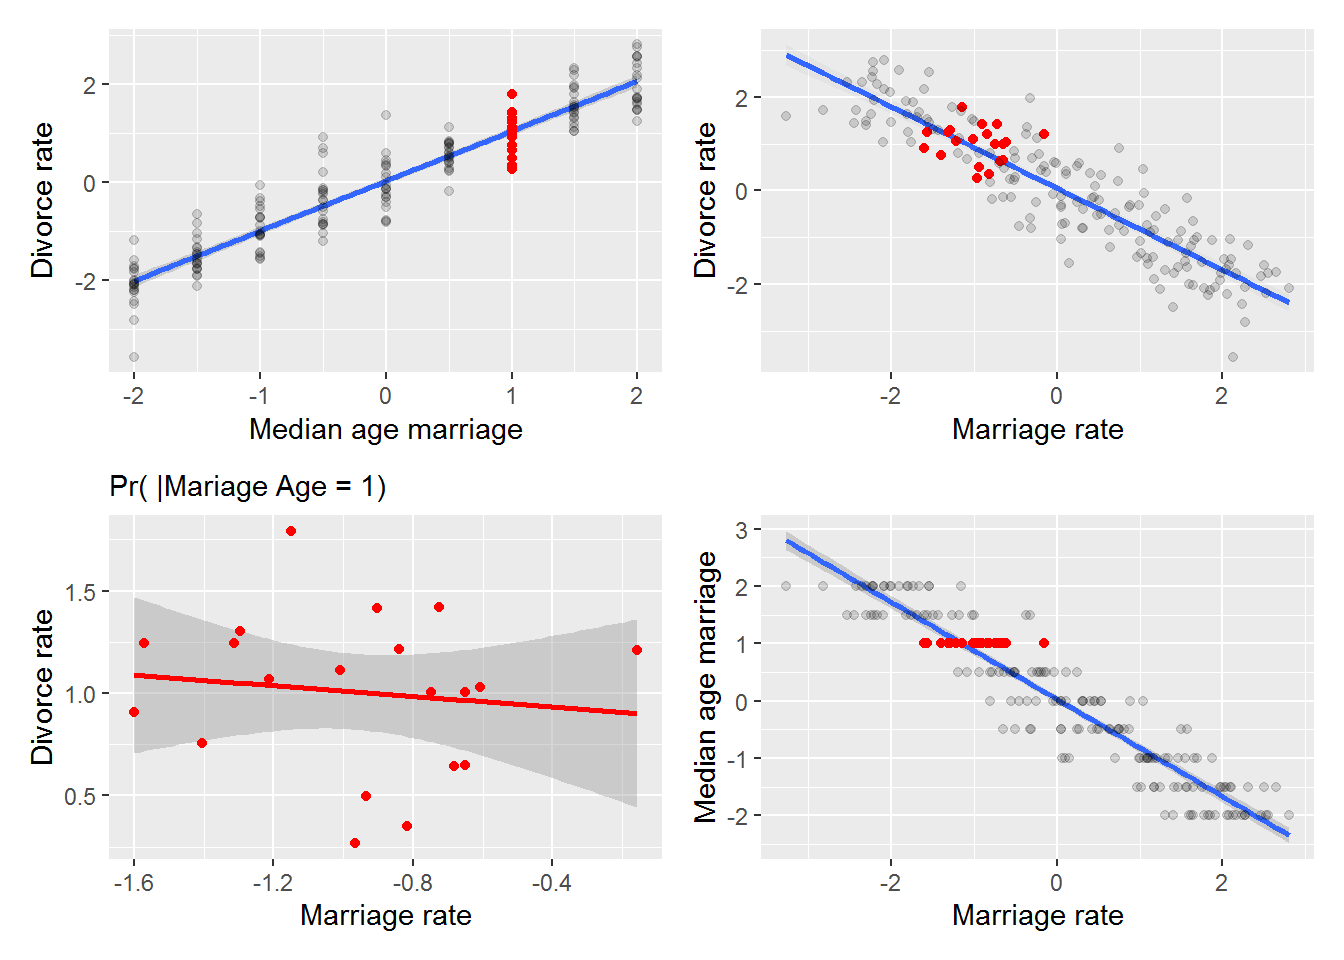
\includegraphics[width=1\linewidth]{notes-on-statistical-rethinking_files/figure-latex/unnamed-chunk-12-1} \end{center}

First, take at top-left and bottom-right plots that plot, correspondingly, divorce and marriage rate versus marriage age. Note that I've flipped axes on the bottom-right plot, so that marriage rate is always mapped on x-axis. The \emph{red} dots in each plot correspond to divorce and marriage rates \emph{given that} (filtered on) marriage age is 1. The same dots are marked in red in the top-right plot and are plotted separately at the bottom-right. As you can see, the two variables \emph{conditional on A=1} are uncorrelated. Why? Because both were fully determined by marriage age and any variation (the spread of red dots vertically or horizontally in the top-left and bottom-right plots) was due to noise. Therefore, the plot on the bottom-left effectively plots noise in marriage rate versus noise in divorce rate and, by our synthetic data design, the noise in two variable was independent, hence, lack of correlation.

This opportunity to turn dependence into independence by conditioning two variables on the third is at the heart of causal reasoning\footnote{As you will learn later, the opposite is also true, so you can turn independence into conditional dependence.}. You draw a DAG and if it has a fork in it, you know that \emph{given your educated guess about causal relationship is correct} (small world!), your data (large world!) should show dependence \emph{and} conditional independence of the two variables (divorce and marriage rates). What if it does not? E.g., the two variables are always dependent or always independent, conditional or not? As we already discussed above, that just means that your educated guess was wrong and that relationship of the variables is different from how you thought it is. Thus, you need to go back to the drawing board, come up with another DAG, repeat the analysis and see if that new DAG is supported by data. If you have more variables, your DAGs will be more complex but the beauty of such causal reasoning is that you can concentrate on \emph{parts} of it, picking three variables and seeing whether your guess about these three variables was correct. This way, you can tinker with your causal model part-by-part, instead of hoping that you got \emph{everything} right on the very first attempt.

\hypertarget{collider-bias}{%
\chapter{Collider bias}\label{collider-bias}}

This notes are on Chapter 5 ``The Many Variables \& The Spurious Waffles'', specifically, on section 5.1 ``Spurious association''. If you are to remember one thing from that chapter, it should be ``doing multiple regression is easy, understanding and interpreting it is hard''. As you will see below, fully understanding relationship between variables is complicate even when we are working with a minimal multiple regression with just two predictors.

When reading section 5.1 ``Spurious association'', I found relationships between the \emph{marriage age}, \emph{marriage rate}, and \emph{divorce rate} to be both clear and mysterious. On the one hand, everything is correlated with everything.

\begin{center}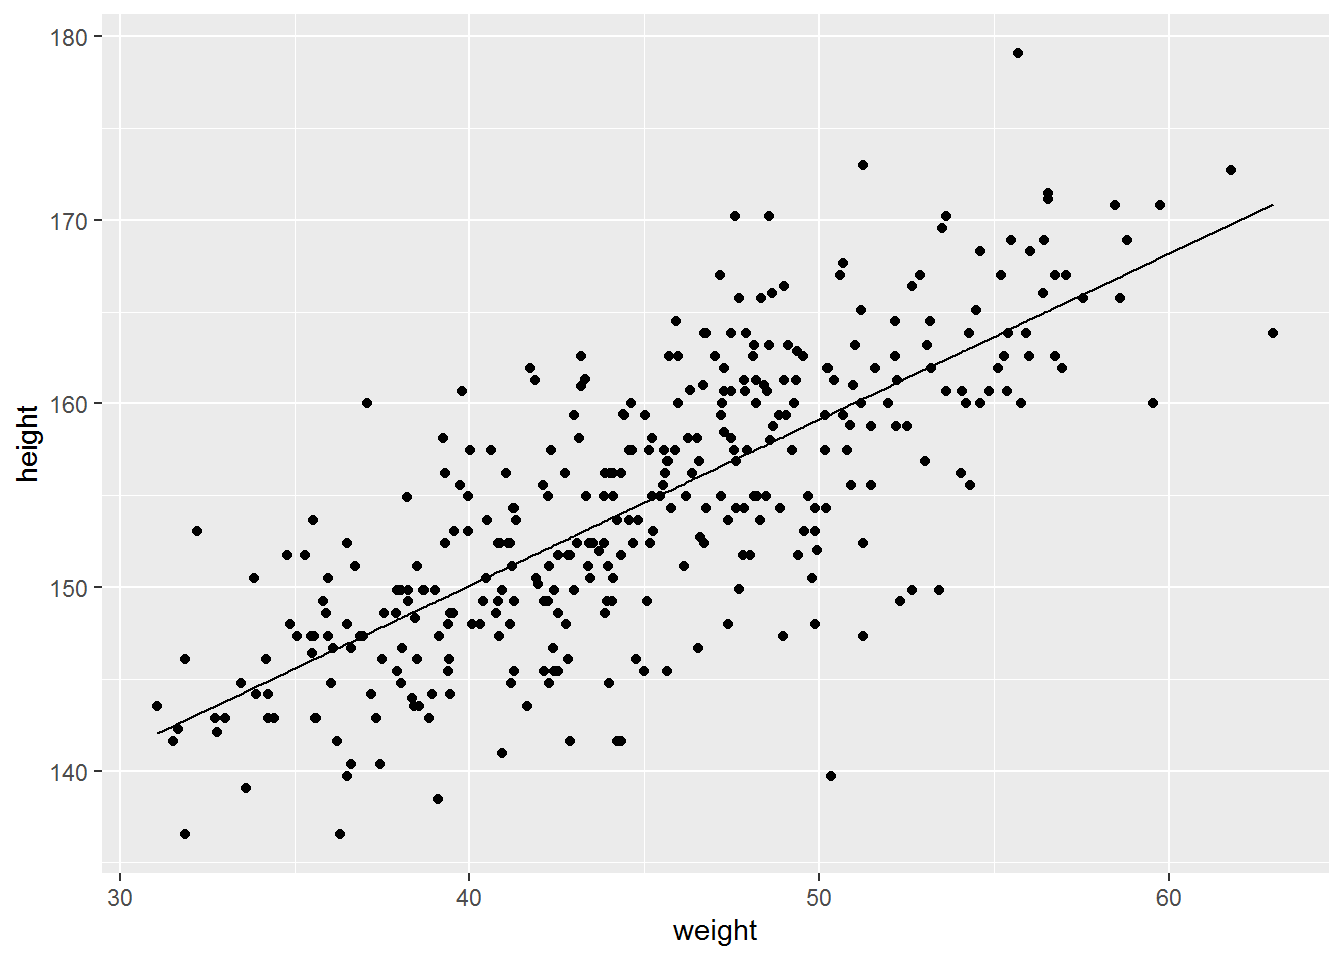
\includegraphics[width=1\linewidth]{notes-on-statistical-rethinking_files/figure-latex/unnamed-chunk-14-1} \end{center}

On the other hand, once we fit linear model to predict divorce rate based on both median age marriage and marriage rate, the latter is \emph{clearly} irrelevant (output of code 5.11 shows that its coefficient is effectively zero, meaning that it is ignored) and, therefore, it has no causal influence on divorce rate.

If you are like me\footnote{Don't be like me, be better!}, you said ``Huh! But how does the model know that?''. And, at least for me, explanations in the chapter did not help much. The key figure is 5.4, that shows that (omitting intercept and slope symbols) \texttt{median\ age\ marriage\ =\ marriage\ rate\ +\ *extra\ information*\ +\ noise} but \texttt{marriage\ rate\ =\ median\ age\ marriage\ +\ noise}. In a nutshell, both variables code the same information but marriage rate is a noisier version of it, so it is ignored. Unfortunately, the answer ``but how?'' still stands. The figure 5.4, which shows fits on residuals is illustrative, but we do not fit residuals, we fit both variables at the same time \emph{without} fitting them on each other! Nowhere in the model 5.1.4 do we find \[\mu^{M}_{i} = \alpha_{AM} + \beta_{AM} * A_i\]

So, what's going on? \emph{How does it know?} To understand this, let us start with an issue of \emph{multicollinearity}.

\hypertarget{multicollinearity}{%
\section{Multicollinearity}\label{multicollinearity}}

To make things easier to understand, let us use simulated data. Imagine that both marriage and divorce rate are both \emph{caused by} marriage age and are almost perfectly linearly dependent it, so that \(D_i = \beta_A^{true} \cdot A_i\) (for the sake of simplicity \(\beta_A^{true} = -1\)) and \(M_i = -A_i\). The \emph{causal} relationship that we are modeling is called a fork:
\[Marriage~rate~\leftarrow~Age~of~marriage~\rightarrow~Divorce~rate\].
We pretend our variables are already standardized, so the plots would look something like this.

\begin{Shaded}
\begin{Highlighting}[]
\FunctionTok{data}\NormalTok{(}\StringTok{"WaffleDivorce"}\NormalTok{)}
\FunctionTok{set.seed}\NormalTok{(}\DecValTok{1212}\NormalTok{)}
\NormalTok{N }\OtherTok{\textless{}{-}} \FunctionTok{nrow}\NormalTok{(WaffleDivorce)}
\NormalTok{sim\_waffles }\OtherTok{\textless{}{-}} \FunctionTok{tibble}\NormalTok{(}\AttributeTok{MedianAgeMarriage =} \FunctionTok{rnorm}\NormalTok{(N),}
                      \AttributeTok{Divorce =} \SpecialCharTok{{-}}\FunctionTok{rnorm}\NormalTok{(N, MedianAgeMarriage, }\FloatTok{0.1}\NormalTok{),}
                      \AttributeTok{Marriage =} \SpecialCharTok{{-}}\FunctionTok{rnorm}\NormalTok{(N, MedianAgeMarriage, }\FloatTok{0.01}\NormalTok{))}

\NormalTok{MD\_plot }\OtherTok{\textless{}{-}} 
  \FunctionTok{ggplot}\NormalTok{(}\AttributeTok{data=}\NormalTok{sim\_waffles, }\FunctionTok{aes}\NormalTok{(}\AttributeTok{x=}\NormalTok{Marriage, }\AttributeTok{y=}\NormalTok{Divorce)) }\SpecialCharTok{+} 
  \FunctionTok{geom\_smooth}\NormalTok{(}\AttributeTok{method=}\StringTok{"lm"}\NormalTok{, }\AttributeTok{formula=}\NormalTok{y}\SpecialCharTok{\textasciitilde{}}\NormalTok{x) }\SpecialCharTok{+} 
  \FunctionTok{geom\_point}\NormalTok{() }\SpecialCharTok{+} 
  \FunctionTok{xlab}\NormalTok{(}\StringTok{"Marriage rate"}\NormalTok{) }\SpecialCharTok{+} 
  \FunctionTok{ylab}\NormalTok{(}\StringTok{"Divorce rate"}\NormalTok{)}

\NormalTok{AD\_plot }\OtherTok{\textless{}{-}} 
  \FunctionTok{ggplot}\NormalTok{(}\AttributeTok{data=}\NormalTok{sim\_waffles, }\FunctionTok{aes}\NormalTok{(}\AttributeTok{x=}\NormalTok{MedianAgeMarriage, }\AttributeTok{y=}\NormalTok{Divorce)) }\SpecialCharTok{+} 
  \FunctionTok{geom\_smooth}\NormalTok{(}\AttributeTok{method=}\StringTok{"lm"}\NormalTok{, }\AttributeTok{formula=}\NormalTok{y}\SpecialCharTok{\textasciitilde{}}\NormalTok{x) }\SpecialCharTok{+} 
  \FunctionTok{geom\_point}\NormalTok{() }\SpecialCharTok{+} 
  \FunctionTok{xlab}\NormalTok{(}\StringTok{"Median age marriage"}\NormalTok{) }\SpecialCharTok{+} 
  \FunctionTok{ylab}\NormalTok{(}\StringTok{"Divorce rate"}\NormalTok{)}

\NormalTok{AM\_plot }\OtherTok{\textless{}{-}} 
  \FunctionTok{ggplot}\NormalTok{(}\AttributeTok{data=}\NormalTok{sim\_waffles, }\FunctionTok{aes}\NormalTok{(}\AttributeTok{x=}\NormalTok{MedianAgeMarriage, }\AttributeTok{y=}\NormalTok{Marriage)) }\SpecialCharTok{+} 
  \FunctionTok{geom\_smooth}\NormalTok{(}\AttributeTok{method=}\StringTok{"lm"}\NormalTok{, }\AttributeTok{formula=}\NormalTok{y}\SpecialCharTok{\textasciitilde{}}\NormalTok{x) }\SpecialCharTok{+} 
  \FunctionTok{geom\_point}\NormalTok{() }\SpecialCharTok{+} 
  \FunctionTok{xlab}\NormalTok{(}\StringTok{"Median age marriage"}\NormalTok{) }\SpecialCharTok{+} 
  \FunctionTok{ylab}\NormalTok{(}\StringTok{"Marriage rate"}\NormalTok{)}

\NormalTok{MD\_plot }\SpecialCharTok{|}\NormalTok{ AD\_plot }\SpecialCharTok{|}\NormalTok{ AM\_plot}
\end{Highlighting}
\end{Shaded}

\begin{center}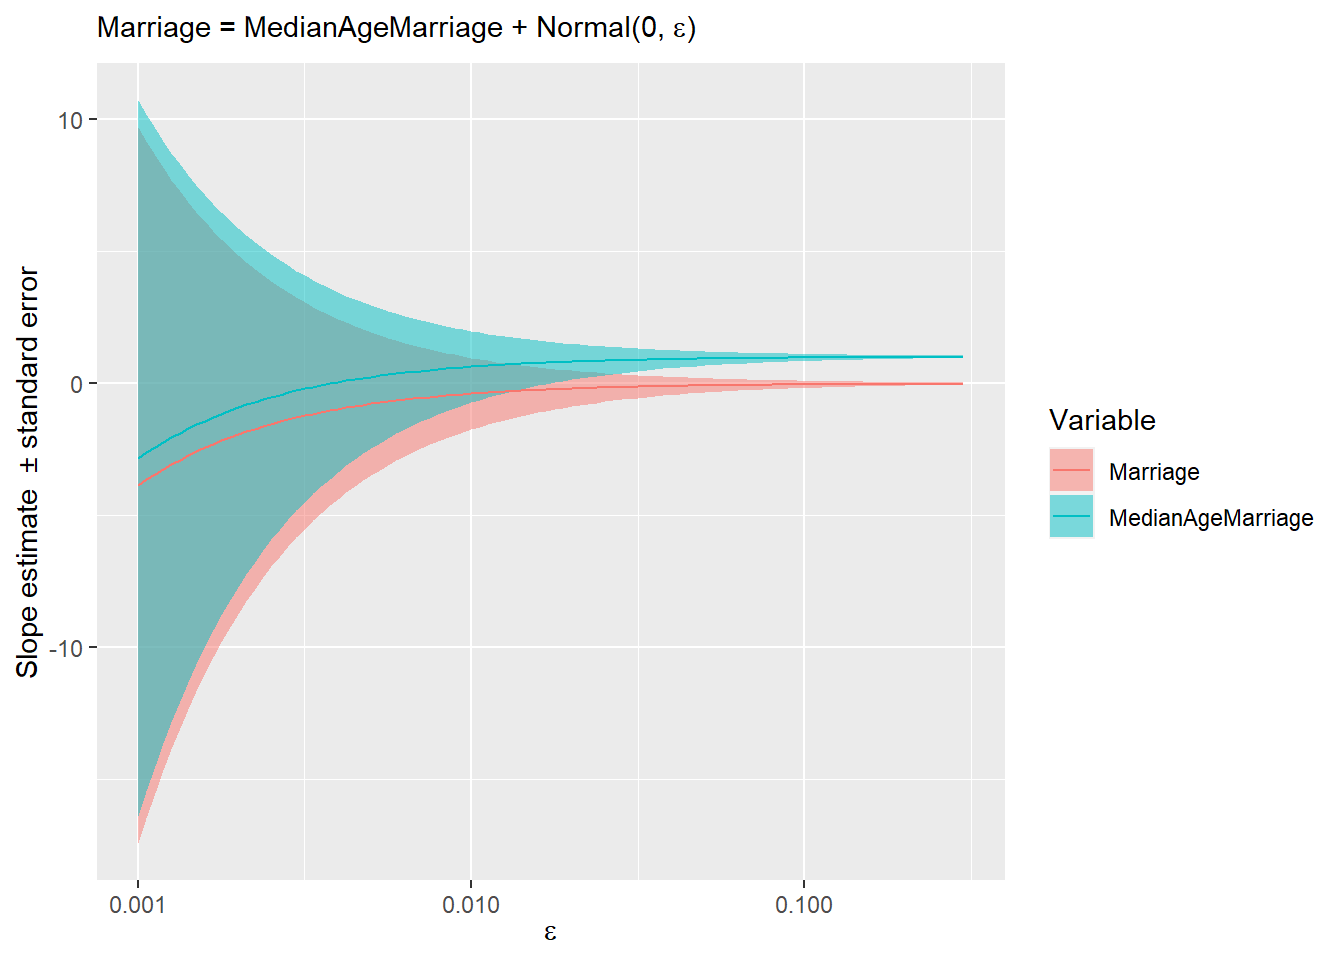
\includegraphics[width=1\linewidth]{notes-on-statistical-rethinking_files/figure-latex/unnamed-chunk-15-1} \end{center}

The relationship is the same as in the plots above but, as we assumed an almost perfect correlation, there is not much spread around the regression line. Still, by definition of \emph{how we constructed the data}, both marriage and divorce rate are \emph{caused} (computed from) median age and, importantly, marriage rate is \emph{never} used to compute the divorce rate. What happens if we analyze this simulated data using the same model 5.1.3, will it be able to figure ``marriage rate does not matter'' again?

\begin{Shaded}
\begin{Highlighting}[]
\NormalTok{sim\_waffles }\OtherTok{\textless{}{-}}
\NormalTok{  sim\_waffles }\SpecialCharTok{\%\textgreater{}\%}
  \FunctionTok{mutate}\NormalTok{(}\AttributeTok{A =}\NormalTok{ MedianAgeMarriage,}
         \AttributeTok{M =}\NormalTok{ Marriage,}
         \AttributeTok{D =}\NormalTok{ Divorce)}

\NormalTok{sim\_waffles\_fit }\OtherTok{\textless{}{-}} \FunctionTok{quap}\NormalTok{(}
  \FunctionTok{alist}\NormalTok{(}
\NormalTok{    D }\SpecialCharTok{\textasciitilde{}} \FunctionTok{dnorm}\NormalTok{(mu , sigma) ,}
\NormalTok{    mu }\OtherTok{\textless{}{-}}\NormalTok{ a }\SpecialCharTok{+}\NormalTok{ bM}\SpecialCharTok{*}\NormalTok{M }\SpecialCharTok{+}\NormalTok{ bA}\SpecialCharTok{*}\NormalTok{A,}
\NormalTok{    a }\SpecialCharTok{\textasciitilde{}} \FunctionTok{dnorm}\NormalTok{(}\DecValTok{0}\NormalTok{, }\FloatTok{0.2}\NormalTok{),}
\NormalTok{    bA }\SpecialCharTok{\textasciitilde{}} \FunctionTok{dnorm}\NormalTok{(}\DecValTok{0}\NormalTok{, }\DecValTok{10}\NormalTok{),}
\NormalTok{    bM }\SpecialCharTok{\textasciitilde{}} \FunctionTok{dnorm}\NormalTok{(}\DecValTok{0}\NormalTok{, }\DecValTok{10}\NormalTok{),}
\NormalTok{    sigma }\SpecialCharTok{\textasciitilde{}} \FunctionTok{dexp}\NormalTok{(}\DecValTok{1}\NormalTok{)}
\NormalTok{  ), }
  \AttributeTok{data =}\NormalTok{ sim\_waffles,}
\NormalTok{)}

\FunctionTok{precis}\NormalTok{(sim\_waffles\_fit)}
\end{Highlighting}
\end{Shaded}

\begin{verbatim}
##              mean          sd        5.5%      94.5%
## a     0.002034578 0.012914402 -0.01860513 0.02267429
## bA    0.267403927 1.188973843 -1.63280591 2.16761377
## bM    1.245792079 1.187211226 -0.65160076 3.14318492
## sigma 0.090129176 0.008996557  0.07575094 0.10450741
\end{verbatim}

Oh no, we broke it! \(\beta_M\) is now about \texttt{1.25} rather than zero and \(\beta_A\) is around \texttt{0.27} rather than \texttt{-1}, as it should. Also note the uncertainty associated with both values, as they both overlap heavily with zero\footnote{I've made priors for both betas broad, so that they are not pushed towards zero too aggressively and uncertainty about them is more evident}. So, the data generation process is the same (\texttt{Divorce\ rate\ ←\ Age\ →\ Marriage\ rate}) and the model is the same (changes to priors have no particular impact in this case) but the ``magic'' of inferring the lack an ``causal arrow'' \texttt{Divorce\ rate\ \ →\ Marriage\ rate} is gone! The \emph{only} difference between the two data sets is extra variance (noise) in marriage rate variable, so let us see how the absence of that extra noise in simulated data breaks the magic.

When two variables, marriage age and rate in our case, are (almost) perfectly correlated (\(M = -A\)), that means that you can substitute one for another. Thus, we can rewrite\footnote{I've dropped likelihood and variance only to compress formulas and shed unimportant details. Adding them does not change the essence.}
\[D = \beta_A \cdot A + \beta_M \cdot M \\
D = \beta_A \cdot A + \beta_M \cdot (-A) \\
D = (\beta_A - \beta_M) \cdot A \\
D = \beta_A^{true} \cdot A\]
where
\[ \beta_A^{true} = (\beta_A - \beta_M)\]

That last bit is the curse of multicollinearity, because if two variable have \emph{the same} information, you are, effectively, fitting their \emph{sum}! This is equivalent to fitting the sum\footnote{in our case, the difference, because we defined that \texttt{M\ =\ -A}.} of coefficients times one of the variables and does not matter which one, since they are identical. We used \texttt{A} because we know that it causes \texttt{M}. If you look at the precis output above, you will see that we did fit the \(\beta_A^{true}\)! Since \texttt{bA\ =\ 0.27} and \texttt{bM\ =\ 1.25}, so plugging them in gives us
\[\beta_A^{true} = \beta_A - \beta_M = 0.27 - 1.25 = -0.98\]

Hey, that is the slope that we used to construct divorce rate, so fitting does work! Moreover, we can see that there is very little uncertainty about \(\beta_A^{true}\)

\begin{Shaded}
\begin{Highlighting}[]
\NormalTok{posterior\_samples }\OtherTok{\textless{}{-}} 
\NormalTok{  rethinking}\SpecialCharTok{::}\FunctionTok{extract.samples}\NormalTok{(sim\_waffles\_fit) }\SpecialCharTok{\%\textgreater{}\%}
  \FunctionTok{mutate}\NormalTok{(}\AttributeTok{bA\_true =}\NormalTok{ bA }\SpecialCharTok{{-}}\NormalTok{ bM)}

\FunctionTok{ggplot}\NormalTok{(posterior\_samples, }\FunctionTok{aes}\NormalTok{(}\AttributeTok{x=}\NormalTok{bA\_true)) }\SpecialCharTok{+} 
  \FunctionTok{geom\_histogram}\NormalTok{(}\AttributeTok{bins=}\DecValTok{100}\NormalTok{) }\SpecialCharTok{+} 
  \FunctionTok{xlab}\NormalTok{(}\StringTok{"bA\_true = bA {-} bM"}\NormalTok{)}
\end{Highlighting}
\end{Shaded}

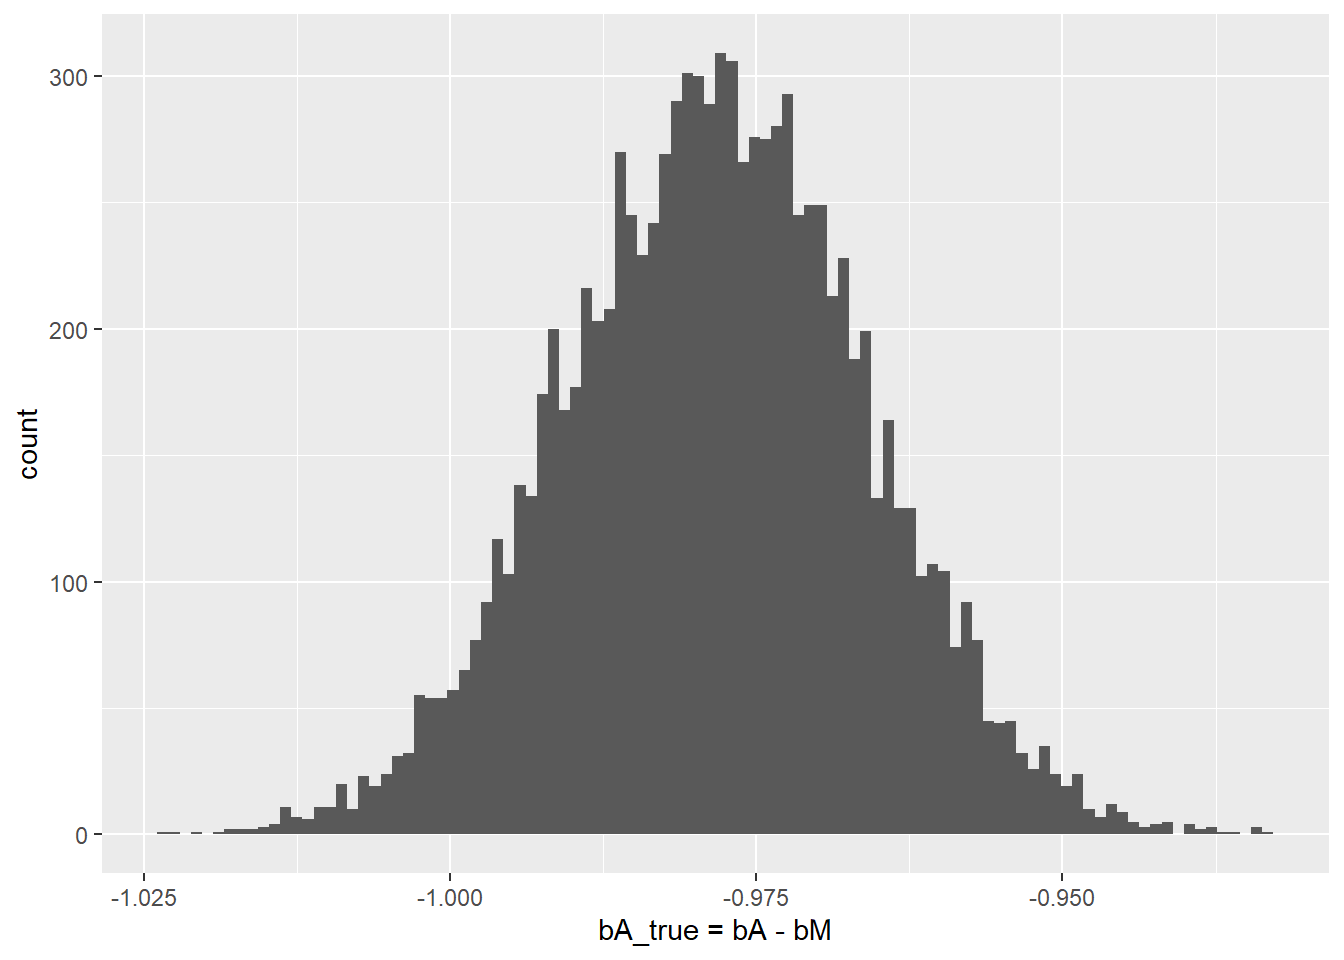
\includegraphics{notes-on-statistical-rethinking_files/figure-latex/unnamed-chunk-17-1.pdf}

But what about uncertainty for \emph{individual} slopes? It stems directly from the fact that \(\beta_A^{true} = \beta_A - \beta_M = -1\) (it is \texttt{-1} in our case, of course). There are infinite number of pairs of numbers whose difference would give -1: \(1-2\), \(2-3\), \((-200)-(-199)\), \(999.41-1000.41\), etc. All of them add up (subtract to) -1, so the fitting procedure cannot settle on any specific region for \emph{each} parameter and any specific pair of values. Any number will do, as long as the \emph{other one} differs by one.

\hypertarget{back-to-spurious-association}{%
\section{Back to spurious association}\label{back-to-spurious-association}}

Above, you have learned that if two variable have the same information, you can only fit \emph{both} of them but cannot get individual slopes. But wasn't that the case for real data we started with? Marriage age and rate \emph{are} correlated, so why fitting used one (age) and not their sum? The answer is \emph{extra noise} in marriage rate. In the real data marriage rate is age \emph{plus some noise}: \(M = -A + \epsilon\), where \(\epsilon\) is traditionally used to denote ``some noise''. How does that extra noise change our linear model for divorce rate?
\[D = \beta_A \cdot A + \beta_M \cdot M \\
D = \beta_A \cdot A + \beta_M (- A + \epsilon) \\
D = (\beta_A  - \beta_M ) \cdot A + \beta_M \cdot \epsilon\]

By definition, \(\epsilon\) is \emph{pure noise} and has zero predictive value with respect to divorce rate. Thus, if we would fit it \emph{alone}, we would expect to get a slope near zero, that is ``no significant relationship''.

\begin{Shaded}
\begin{Highlighting}[]
\FunctionTok{set.seed}\NormalTok{(}\DecValTok{1231455}\NormalTok{)}
\NormalTok{sim\_waffles }\OtherTok{\textless{}{-}} \FunctionTok{tibble}\NormalTok{(}\AttributeTok{MedianAgeMarriage =} \FunctionTok{rnorm}\NormalTok{(N),}
                      \AttributeTok{Divorce =} \FunctionTok{rnorm}\NormalTok{(N, MedianAgeMarriage, }\FloatTok{0.1}\NormalTok{),}
                      \AttributeTok{Marriage =} \SpecialCharTok{{-}}\FunctionTok{rnorm}\NormalTok{(N, MedianAgeMarriage, }\FloatTok{0.01}\NormalTok{),}
                      \AttributeTok{epsilon =} \FunctionTok{rnorm}\NormalTok{(N))}

\FunctionTok{ggplot}\NormalTok{(sim\_waffles, }\FunctionTok{aes}\NormalTok{(}\AttributeTok{x=}\NormalTok{epsilon, }\AttributeTok{y=}\NormalTok{Divorce)) }\SpecialCharTok{+} 
  \FunctionTok{geom\_smooth}\NormalTok{(}\AttributeTok{method=}\StringTok{"lm"}\NormalTok{, }\AttributeTok{formula=}\NormalTok{y}\SpecialCharTok{\textasciitilde{}}\NormalTok{x) }\SpecialCharTok{+} 
  \FunctionTok{geom\_point}\NormalTok{() }\SpecialCharTok{+} 
  \FunctionTok{xlab}\NormalTok{(}\FunctionTok{expression}\NormalTok{(epsilon)) }\SpecialCharTok{+} 
  \FunctionTok{ylab}\NormalTok{(}\StringTok{"Marriage rate"}\NormalTok{)}
\end{Highlighting}
\end{Shaded}

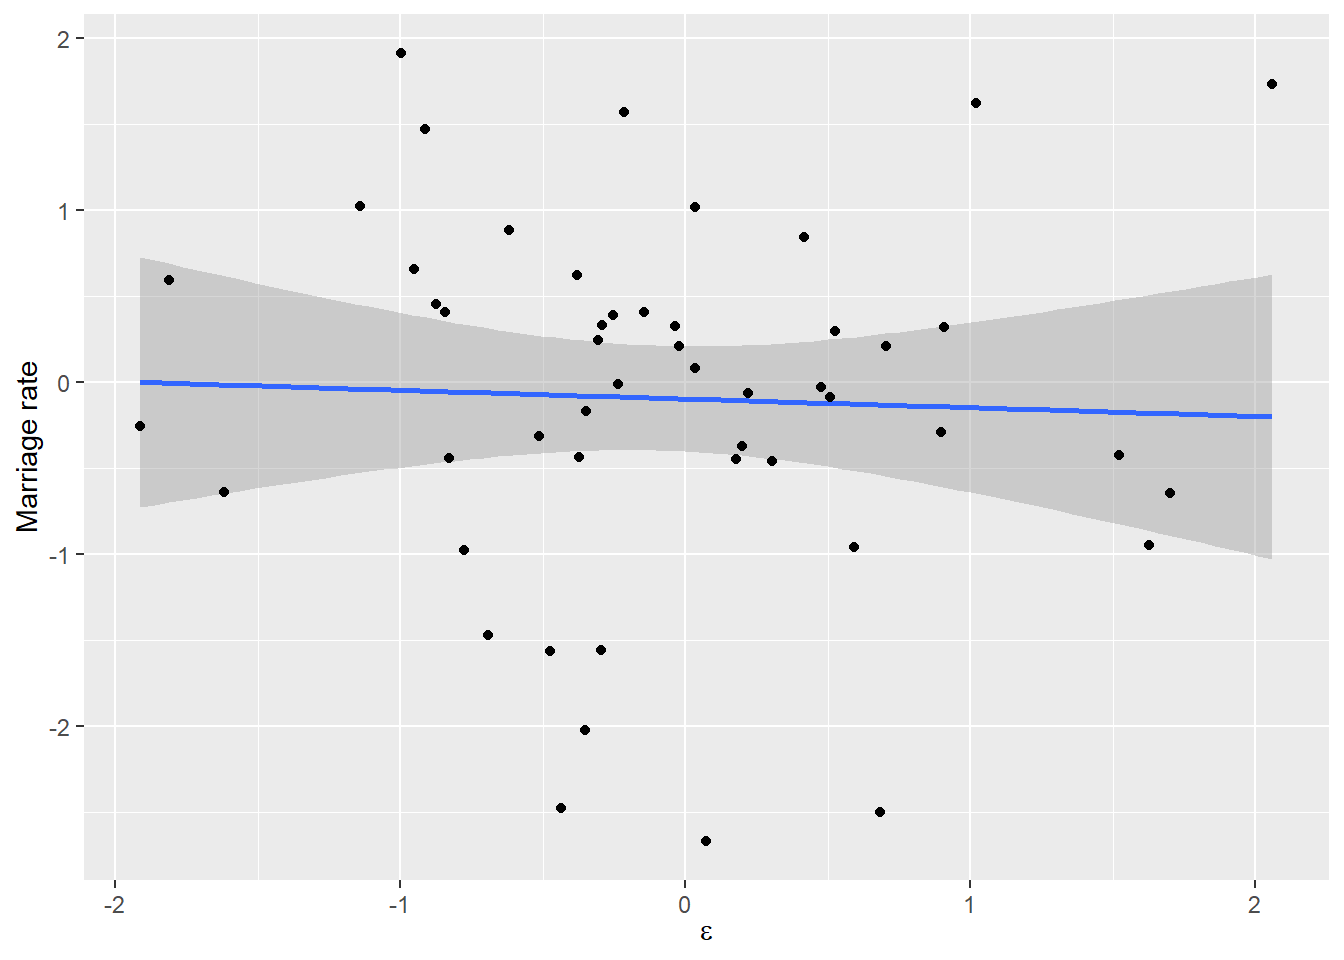
\includegraphics{notes-on-statistical-rethinking_files/figure-latex/unnamed-chunk-18-1.pdf}

But we are not fitting it alone, as the coefficient \(\beta_M\) appears at \emph{twice}:
\[D = (\beta_A  - \beta_M) \cdot A + \beta_M \cdot \epsilon\]
The latter part, \(\beta_M \cdot \epsilon\), pushes \(\beta_M\) towards zero slope, which is the best solution for pure noise, as you saw in the plot above. But the former part, \(\beta_A - \beta_M\) only needs to add up to \(\beta_A^{true}\), so however we fix \(\beta_M\), \(\beta_A\) can accommodate. Thus the closer \(\beta_M\) to zero, the closer is \(\beta_A\) to \(\beta_A^{true}\). And that's how the magic works! If one variable is other variable plus noise, that \emph{plus noise} induces extra penalty (extra residuals) and the only way to reduce residuals is to ignore the \emph{uncorrelated} noise by setting the slope to zero. Therefore, you ignore the variable as well, because it is merely a noisy twin of a better variable. You can see how added noise ``disambiguates'' the causal relationship\footnote{I've used ordinary least squares just to make simulations faster. You will get the same result using Bayesian fittings procedures.}.

\begin{Shaded}
\begin{Highlighting}[]
\NormalTok{simulate\_waffles }\OtherTok{\textless{}{-}} \ControlFlowTok{function}\NormalTok{(sigma\_noise)\{}
  \CommentTok{\# generate same data but for noise in Marraige from Age relationship}
  \FunctionTok{set.seed}\NormalTok{(}\DecValTok{169084}\NormalTok{)}
\NormalTok{  sim\_df }\OtherTok{\textless{}{-}}\NormalTok{ sim\_waffles }\OtherTok{\textless{}{-}} \FunctionTok{tibble}\NormalTok{(}\AttributeTok{MedianAgeMarriage =} \FunctionTok{rnorm}\NormalTok{(N),}
                                  \AttributeTok{Divorce =} \FunctionTok{rnorm}\NormalTok{(N, MedianAgeMarriage, }\FloatTok{0.1}\NormalTok{),}
                                  \AttributeTok{Marriage =} \SpecialCharTok{{-}}\FunctionTok{rnorm}\NormalTok{(N, MedianAgeMarriage, sigma\_noise))}
  
  \CommentTok{\# fit data using OLS and pulling out two slope coefficients}
  \FunctionTok{lm}\NormalTok{(Divorce }\SpecialCharTok{\textasciitilde{}}\NormalTok{ Marriage }\SpecialCharTok{+}\NormalTok{ MedianAgeMarriage, }\AttributeTok{data=}\NormalTok{sim\_df) }\SpecialCharTok{\%\textgreater{}\%} 
    \FunctionTok{summary}\NormalTok{() }\SpecialCharTok{\%\textgreater{}\%}
\NormalTok{    .}\SpecialCharTok{$}\NormalTok{coefficients }\SpecialCharTok{\%\textgreater{}\%}
    \FunctionTok{data.frame}\NormalTok{() }\SpecialCharTok{\%\textgreater{}\%}
    \FunctionTok{rownames\_to\_column}\NormalTok{(}\StringTok{"Variable"}\NormalTok{) }\SpecialCharTok{\%\textgreater{}\%}
    \FunctionTok{slice}\NormalTok{(}\SpecialCharTok{{-}}\DecValTok{1}\NormalTok{) }\SpecialCharTok{\%\textgreater{}\%}
    \FunctionTok{mutate}\NormalTok{(}\AttributeTok{LowerCI =}\NormalTok{ Estimate }\SpecialCharTok{{-}}\NormalTok{ Std..Error,}
           \AttributeTok{UpperCI =}\NormalTok{ Estimate }\SpecialCharTok{+}\NormalTok{ Std..Error) }\SpecialCharTok{\%\textgreater{}\%}
    \FunctionTok{select}\NormalTok{(Variable, Estimate, LowerCI, UpperCI)}
\NormalTok{\}}

\NormalTok{simulated\_noise }\OtherTok{\textless{}{-}} 
  \FunctionTok{tibble}\NormalTok{(}\AttributeTok{epsilon =}\FunctionTok{exp}\NormalTok{(}\FunctionTok{seq}\NormalTok{(}\FunctionTok{log}\NormalTok{(}\FloatTok{0.001}\NormalTok{), }\FunctionTok{log}\NormalTok{(}\FloatTok{0.3}\NormalTok{), }\AttributeTok{length.out =} \DecValTok{100}\NormalTok{))) }\SpecialCharTok{\%\textgreater{}\%}
  \FunctionTok{group\_by}\NormalTok{(epsilon) }\SpecialCharTok{\%\textgreater{}\%}
  \FunctionTok{do}\NormalTok{(}\FunctionTok{simulate\_waffles}\NormalTok{(.}\SpecialCharTok{$}\NormalTok{epsilon))}

\FunctionTok{ggplot}\NormalTok{(simulated\_noise, }\FunctionTok{aes}\NormalTok{(}\AttributeTok{x=}\NormalTok{epsilon, }\AttributeTok{y=}\NormalTok{Estimate)) }\SpecialCharTok{+} 
  \FunctionTok{geom\_ribbon}\NormalTok{(}\FunctionTok{aes}\NormalTok{(}\AttributeTok{ymin=}\NormalTok{LowerCI, }\AttributeTok{ymax=}\NormalTok{UpperCI, }\AttributeTok{fill=}\NormalTok{Variable), }\AttributeTok{alpha=} \FloatTok{0.5}\NormalTok{) }\SpecialCharTok{+} 
  \FunctionTok{geom\_line}\NormalTok{(}\FunctionTok{aes}\NormalTok{(}\AttributeTok{color=}\NormalTok{Variable)) }\SpecialCharTok{+} 
  \FunctionTok{scale\_x\_log10}\NormalTok{(}\AttributeTok{name=}\FunctionTok{expression}\NormalTok{(epsilon)) }\SpecialCharTok{+} 
  \FunctionTok{ylab}\NormalTok{(}\StringTok{"Slope estimate  ± standard error"}\NormalTok{) }\SpecialCharTok{+}
  \FunctionTok{labs}\NormalTok{(}\AttributeTok{subtitle =} \FunctionTok{expression}\NormalTok{(}\FunctionTok{paste}\NormalTok{(}\StringTok{"Marriage = MedianAgeMarriage + Normal(0, "}\NormalTok{, epsilon, }\StringTok{")"}\NormalTok{)))}
\end{Highlighting}
\end{Shaded}

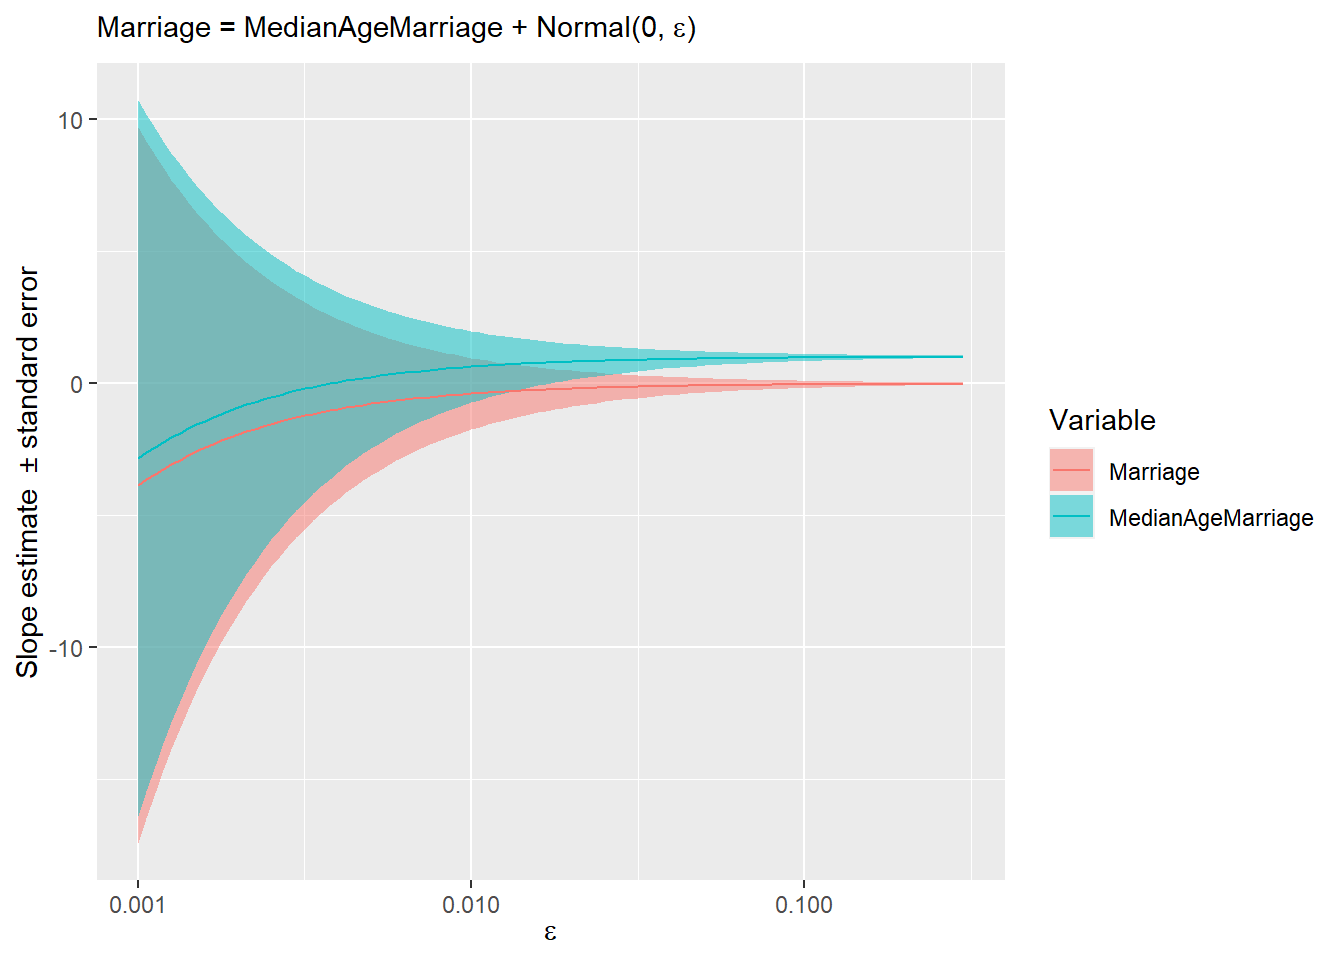
\includegraphics{notes-on-statistical-rethinking_files/figure-latex/unnamed-chunk-19-1.pdf}

The stripes show uncertainty (estimate ± standard error) and you can appreciate how quickly it is reduced as marriage rate becomes noisier and just how little noise is required for ``magic'' to start working and converge on the true causal relationship\footnote{It is true only in a sense that it matches the processes of creating the data. It is \emph{not} necessarily truly true for real data!}.

\hypertarget{chain-dag}{%
\section{Chain DAG}\label{chain-dag}}

So, a bit of noise will fix everything and we can \emph{know} causal relationships between the three variables? Not necessarily! Consider another possible causal diagram:
\[Marriage~rate~\rightarrow~Age~of~marriage~\rightarrow~Divorce~rate\]
Now marriage rate causes age of marriage that, in turn, causes divorce rate. Again, let us use synthetic data, so that we can be sure what causes what. However, we will add a fair amount of noise to make it more like real data and avoid multicoliniarity.

\begin{Shaded}
\begin{Highlighting}[]
\FunctionTok{data}\NormalTok{(}\StringTok{"WaffleDivorce"}\NormalTok{)}
\FunctionTok{set.seed}\NormalTok{(}\DecValTok{8973791}\NormalTok{)}
\NormalTok{N }\OtherTok{\textless{}{-}} \FunctionTok{nrow}\NormalTok{(WaffleDivorce)}
\NormalTok{sim\_waffles }\OtherTok{\textless{}{-}} \FunctionTok{tibble}\NormalTok{(}\AttributeTok{Marriage =} \FunctionTok{rnorm}\NormalTok{(N),}
                      \AttributeTok{MedianAgeMarriage =} \SpecialCharTok{{-}}\FunctionTok{rnorm}\NormalTok{(N, Marriage, }\FloatTok{0.2}\NormalTok{),}
                      \AttributeTok{Divorce =} \SpecialCharTok{{-}}\FunctionTok{rnorm}\NormalTok{(N, MedianAgeMarriage, }\FloatTok{0.2}\NormalTok{))}

\NormalTok{MD\_plot }\OtherTok{\textless{}{-}} 
  \FunctionTok{ggplot}\NormalTok{(}\AttributeTok{data=}\NormalTok{sim\_waffles, }\FunctionTok{aes}\NormalTok{(}\AttributeTok{x=}\NormalTok{Marriage, }\AttributeTok{y=}\NormalTok{Divorce)) }\SpecialCharTok{+} 
  \FunctionTok{geom\_smooth}\NormalTok{(}\AttributeTok{method=}\StringTok{"lm"}\NormalTok{, }\AttributeTok{formula=}\NormalTok{y}\SpecialCharTok{\textasciitilde{}}\NormalTok{x) }\SpecialCharTok{+} 
  \FunctionTok{geom\_point}\NormalTok{() }\SpecialCharTok{+} 
  \FunctionTok{xlab}\NormalTok{(}\StringTok{"Marriage rate"}\NormalTok{) }\SpecialCharTok{+} 
  \FunctionTok{ylab}\NormalTok{(}\StringTok{"Divorce rate"}\NormalTok{)}

\NormalTok{AD\_plot }\OtherTok{\textless{}{-}} 
  \FunctionTok{ggplot}\NormalTok{(}\AttributeTok{data=}\NormalTok{sim\_waffles, }\FunctionTok{aes}\NormalTok{(}\AttributeTok{x=}\NormalTok{MedianAgeMarriage, }\AttributeTok{y=}\NormalTok{Divorce)) }\SpecialCharTok{+} 
  \FunctionTok{geom\_smooth}\NormalTok{(}\AttributeTok{method=}\StringTok{"lm"}\NormalTok{, }\AttributeTok{formula=}\NormalTok{y}\SpecialCharTok{\textasciitilde{}}\NormalTok{x) }\SpecialCharTok{+} 
  \FunctionTok{geom\_point}\NormalTok{() }\SpecialCharTok{+} 
  \FunctionTok{xlab}\NormalTok{(}\StringTok{"Median age marriage"}\NormalTok{) }\SpecialCharTok{+} 
  \FunctionTok{ylab}\NormalTok{(}\StringTok{"Divorce rate"}\NormalTok{)}

\NormalTok{AM\_plot }\OtherTok{\textless{}{-}} 
  \FunctionTok{ggplot}\NormalTok{(}\AttributeTok{data=}\NormalTok{sim\_waffles, }\FunctionTok{aes}\NormalTok{(}\AttributeTok{x=}\NormalTok{MedianAgeMarriage, }\AttributeTok{y=}\NormalTok{Marriage)) }\SpecialCharTok{+} 
  \FunctionTok{geom\_smooth}\NormalTok{(}\AttributeTok{method=}\StringTok{"lm"}\NormalTok{, }\AttributeTok{formula=}\NormalTok{y}\SpecialCharTok{\textasciitilde{}}\NormalTok{x) }\SpecialCharTok{+} 
  \FunctionTok{geom\_point}\NormalTok{() }\SpecialCharTok{+} 
  \FunctionTok{xlab}\NormalTok{(}\StringTok{"Median age marriage"}\NormalTok{) }\SpecialCharTok{+} 
  \FunctionTok{ylab}\NormalTok{(}\StringTok{"Marriage rate"}\NormalTok{)}

\NormalTok{MD\_plot }\SpecialCharTok{|}\NormalTok{ AD\_plot }\SpecialCharTok{|}\NormalTok{ AM\_plot}
\end{Highlighting}
\end{Shaded}

\begin{center}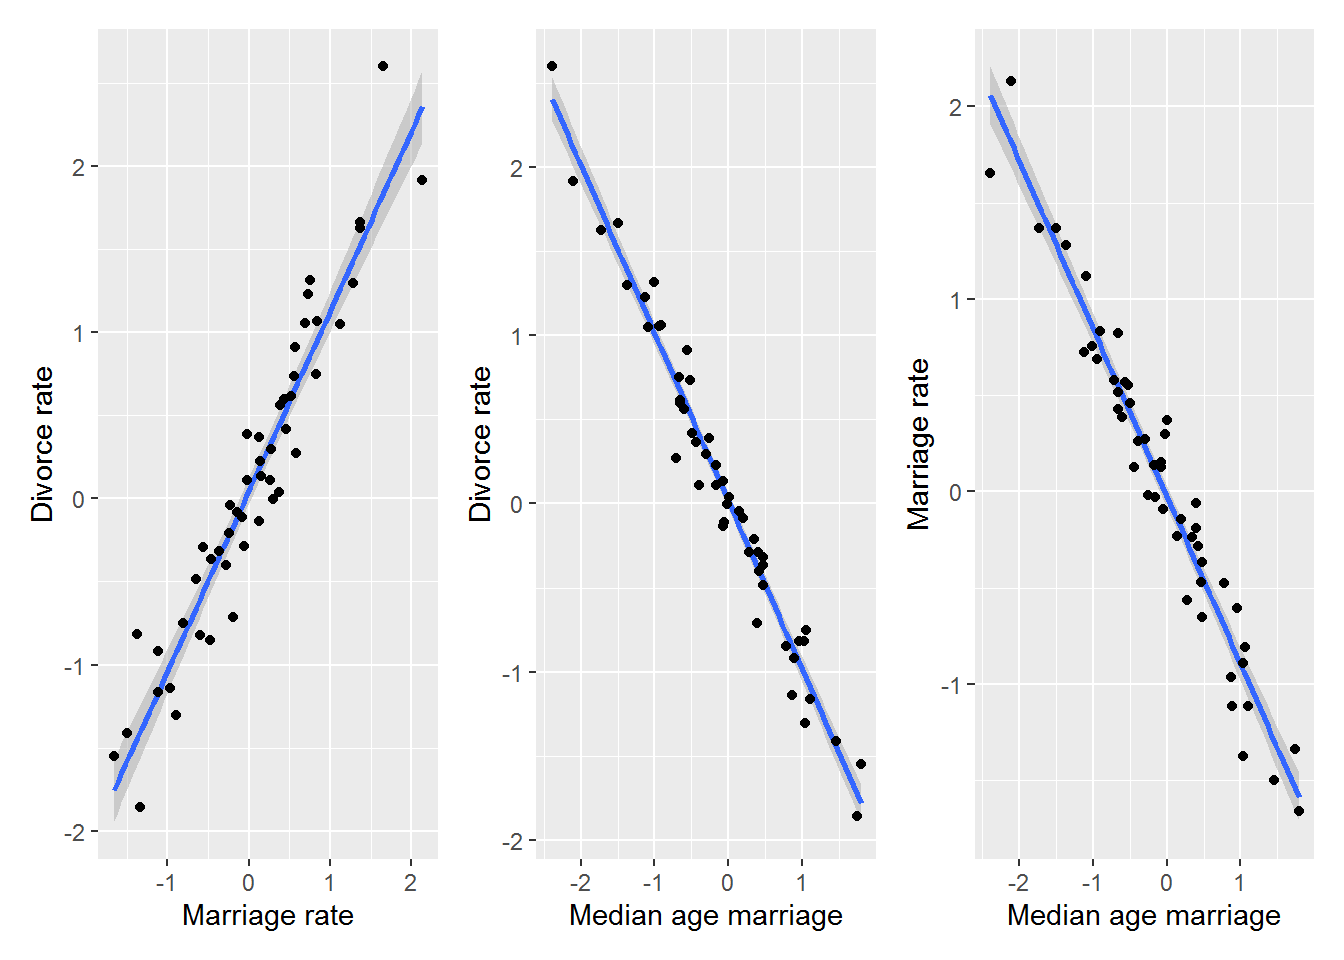
\includegraphics[width=1\linewidth]{notes-on-statistical-rethinking_files/figure-latex/unnamed-chunk-20-1} \end{center}

The plots look very similar to those that we had before, so let us run the model.

\begin{Shaded}
\begin{Highlighting}[]
\NormalTok{sim\_waffles }\OtherTok{\textless{}{-}}
\NormalTok{  sim\_waffles }\SpecialCharTok{\%\textgreater{}\%}
  \FunctionTok{mutate}\NormalTok{(}\AttributeTok{A =}\NormalTok{ MedianAgeMarriage,}
         \AttributeTok{M =}\NormalTok{ Marriage,}
         \AttributeTok{D =}\NormalTok{ Divorce)}

\NormalTok{sim\_waffles\_fit }\OtherTok{\textless{}{-}} \FunctionTok{quap}\NormalTok{(}
  \FunctionTok{alist}\NormalTok{(}
\NormalTok{    D }\SpecialCharTok{\textasciitilde{}} \FunctionTok{dnorm}\NormalTok{(mu , sigma) ,}
\NormalTok{    mu }\OtherTok{\textless{}{-}}\NormalTok{ a }\SpecialCharTok{+}\NormalTok{ bM}\SpecialCharTok{*}\NormalTok{M }\SpecialCharTok{+}\NormalTok{ bA}\SpecialCharTok{*}\NormalTok{A,}
\NormalTok{    a }\SpecialCharTok{\textasciitilde{}} \FunctionTok{dnorm}\NormalTok{(}\DecValTok{0}\NormalTok{, }\FloatTok{0.2}\NormalTok{),}
\NormalTok{    bA }\SpecialCharTok{\textasciitilde{}} \FunctionTok{dnorm}\NormalTok{(}\DecValTok{0}\NormalTok{, }\DecValTok{10}\NormalTok{),}
\NormalTok{    bM }\SpecialCharTok{\textasciitilde{}} \FunctionTok{dnorm}\NormalTok{(}\DecValTok{0}\NormalTok{, }\DecValTok{10}\NormalTok{),}
\NormalTok{    sigma }\SpecialCharTok{\textasciitilde{}} \FunctionTok{dexp}\NormalTok{(}\DecValTok{1}\NormalTok{)}
\NormalTok{  ), }
  \AttributeTok{data =}\NormalTok{ sim\_waffles,}
\NormalTok{)}

\FunctionTok{precis}\NormalTok{(sim\_waffles\_fit)}
\end{Highlighting}
\end{Shaded}

\begin{verbatim}
##              mean         sd        5.5%       94.5%
## a      0.01141493 0.02370058 -0.02646318  0.04929304
## bA    -1.04399582 0.11019913 -1.22011532 -0.86787631
## bM    -0.05011269 0.12299879 -0.24668851  0.14646313
## sigma  0.16656407 0.01661272  0.14001374  0.19311440
\end{verbatim}

The model fit is virtually identical to that for the real data and, effectively, for a noisy simulated fork DAG. Yet, remember, that the underlying causal relationship between marriage rate and marriage age are now \emph{opposite}. In the fork DAG, age was causing marriage rate. Here, in the chain DAG, marriage rate for causing age. Moreover, the way we generated synthetic data, marriage rate causes divorce rate, although its effect is \emph{mediated} via marriage age. Yet, looking at the parameter values for \(\beta_M\) we might be tempted to conclude that marriage rate has no effect on divorce rate. To understand why, think about the relationship between marriage rate and age again. We designed it, so that \(A = -M + \epsilon\) and \(D = -A\) (we ignore the noise in the latter part for clarity). Substituting, we get \(D = M - \epsilon\) or, since we designed noise to be symmetric, we can also write \(D = M + \epsilon\). To put it differently, divorce rate are based on \emph{actual} values of age, which include noise. So, somewhat paradoxically, the cleaner version of the original variable is less correlated. If it still unclear, let me try with a metaphor. Imagine your friend sings you a song she heard. \(original \rightarrow friend \rightarrow you\). She remembered it wrong, so her version is somewhat different from the original. But because you are used to \emph{her} version of the song, the original, once you finally hear it, sounds wrong, as it does not have the distortions introduced by your friend.

\hypertarget{take-home-message}{%
\section{Take-home message}\label{take-home-message}}

So, two DAGs, two \emph{differently} generated data sets, yet, one statistical model. Both DAGs agree that there is a direct causal path between marriage age and divorce but have opposite assumptions about causal relationship between marriage age and rate. What should we conclude from this? That it might be impossible to understand causal relationships between all variables even for the simplest case of just two predictors. The only thing to do is to embrace this ambiguity and be aware of it whenever you interpret regression models. So, you should use DAGs exactly for this purpose of understanding in how many ways can you generate the observed data. I understand that a simple unambiguous story is far more appealing\footnote{``Just tell me how things are!''} but as Jochen Braun of Magdeburg says: ``Do not fall for your own propaganda!''. Selecting just one story / DAG does not make them true. Considering all possible DAGs will likely lead to insights based on predictions they make. Even if your current data cannot decide between them, their different predictions for future experiment will help to solve the puzzle eventually.

Another take home message: Regression models cannot do magic. They can quantify correctional relationship and their signal-to-noise ratios but they do not know causality and they won't tell you which model is the ``true'' model. Imagine that we never measured marriage age, we would model divorce rate from marriage rate and would be quite pleased with the results. And, given how noisy the real data is, we probably did not consider some other \emph{very important} variables, those presence might render age as irrelevant as the marriage rate is now. Again, assuming the chain DAG
\[marriage~rate \rightarrow age \rightarrow variable~we~missed \rightarrow divorce~rate\]
Statistical models only work in a small world you created for them. Models are golems, they cannot and do not know about the large world. You do, so it is on you to understand both their limitations and power. Models can help you understand the process you are investigating but they won't understand it for you!

\hypertarget{the-haunted-dag}{%
\chapter{The haunted DAG}\label{the-haunted-dag}}

These are notes on section \textbf{6.3.2 The haunted DAG} that demonstrates how collider bias can arise, if one of the variables is unobserved and we do not realize that the have a collider in our DAG. The DAG itself is below, I've only changed \texttt{Unobserved} into \texttt{Neighborhood}.

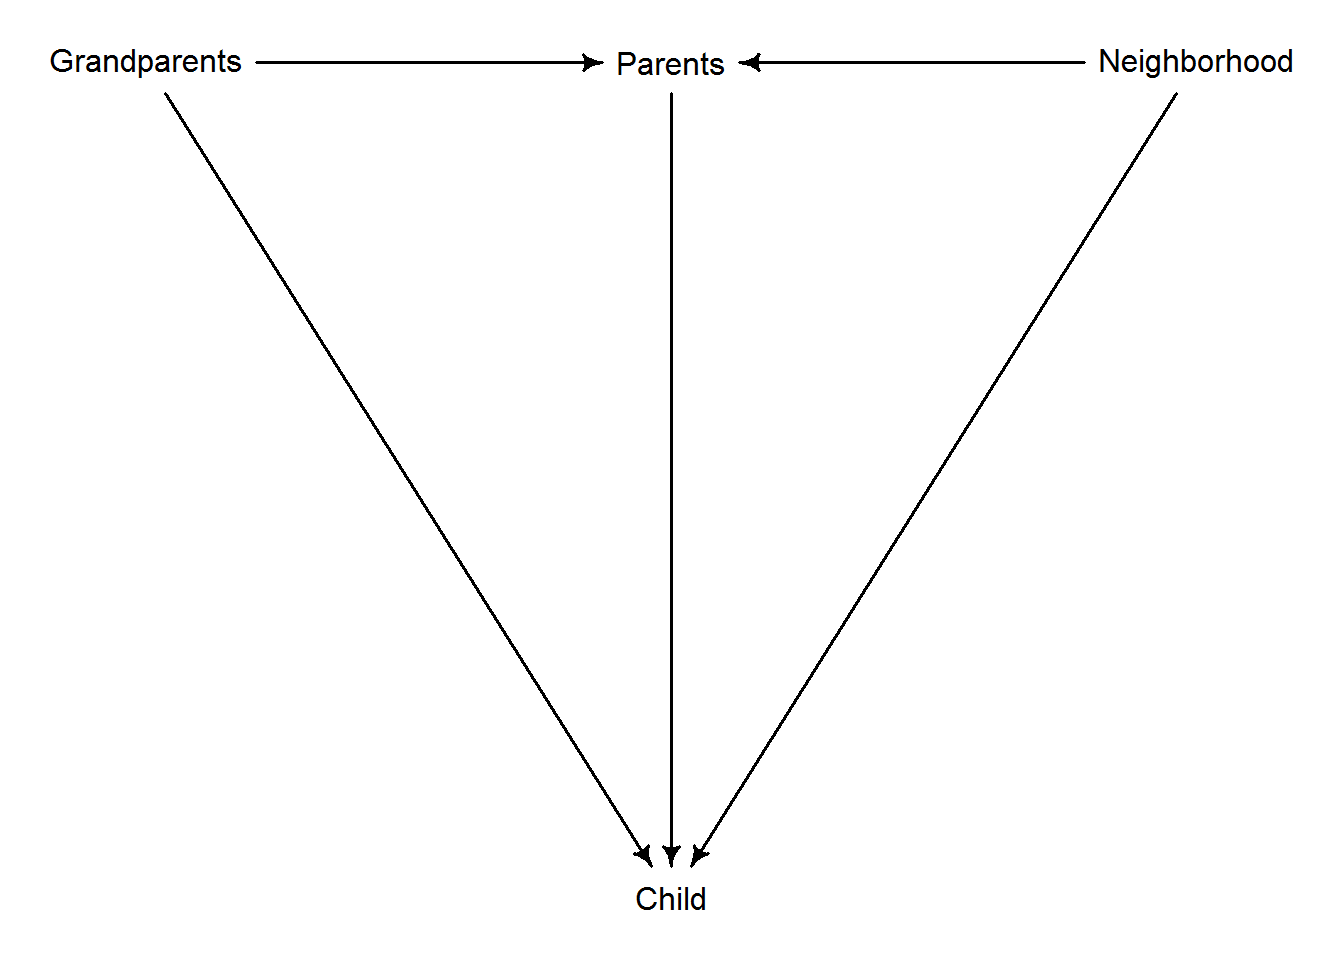
\includegraphics{notes-on-statistical-rethinking_files/figure-latex/unnamed-chunk-23-1.pdf}

The example in the book shows that if we include \texttt{Grandparents} while ``controlling for'' influence of \texttt{Parents} but ignore influence of the \texttt{Neighborhood}, the influence of \texttt{Grandparents} is \emph{negative} rather than \emph{zero}. It is zero in the book but it can originally be positive or negative, point is it is different from what is inferred by the model. And, importantly, an estimated effect of \texttt{Parents} is also different from its true value. The book shows it visually but I found that in this case algebra is helpful to understand it at the level of ``how does a regression model know''.

Let us start with a \emph{full} model. For the sake of simplicity, we will ignore coefficients for computing \texttt{Parents} variable from \texttt{Grandparents} and \texttt{Neighborhood} but this does not change the general picture.

\[ P = G + N\]
Thus, the linear model for child education is
\[C = \beta_P P + \beta_G G + \beta_N N\]

Substituting \$ P = G + N\$ gives us
\[C = \beta_P (G + N) + \beta_G G + \beta_N N\]

Rearranging terms a little
\[C = (\beta_P + \beta_G) G + (\beta_P  + \beta_N) N\]

Note that this means that we do not fit individual coefficients, in both cases we fit a \emph{sum} of two. And, as with multicollinearity, individual coefficients can be in a wrong place and unreliable as long as they add up to the ``true'' coefficient value. Thus, ignoring the noise and concealing the effect of \texttt{Parents}, we might as well fit
\[C = \beta_G^\prime G + \beta_N^\prime N\]
where, \(\beta_G^\prime = \beta_P + \beta_G\) and \(\beta_N^\prime = \beta_P + \beta_N\) are the total effect of grandparents and neighborhood of child education.

What if we ignore \texttt{Neighborhood}? This means that we explicitly set \(\beta_N = 0\) and that is the point when the sum of coefficients starts causing us problems. Recall that the model fits \(\beta_P + \beta_N\) and not each term separately. Thus, setting one of them to 0 does not upset the model, as it can always compensate with the \emph{other} coefficient. Here, that \emph{other} coefficient is \(\beta_P\), so its value now is that of the ``true'' sum: \(\beta_P = \beta_P^{true} + \beta_N^{true}\).

Unfortunately for us, \(\beta_P\) appears at \emph{two} places, as it is also used to quantify effect of grandparents:
\[(\beta_P + \beta_G) G\]

Originally, it reflected only the influence of parents, so it was not a problem. But now it is artificially inflated \footnote{In general, changed depending on the effect signs of individual effects.} as it stands for influence of both parents \emph{and} neighborhood. Problem? Not for a model that fits a \emph{sum}. How do you make sure that \emph{the sum} still adds up? You change \emph{other} coefficients! Here, we can still wiggle \(\beta_G\) so that everything adds up. Given that
\[\beta_P = \beta_P^{true} + \beta_N^{true}\]
model just needs to subtract that same \(\beta_N^{true}\) and get our sum back. So
\[\beta_P + \beta_G = (\beta_P^{true} + \beta_N^{true}) + (\beta_G^{true} - \beta_N^{true})\]

Thus, if we do not explicitly model the effect of neighborhood, it sneaks in nonetheless, hiding inside \emph{both} parent and grandparent coefficients. What makes it really problematic and confusing is that the effect is \emph{opposite} for the two terms: if we \emph{add} \(\beta_N^{true}\) at one place, we must \emph{subtract} it at the other.

So, what are you supposed to do with this new knowledge? You do not take fitted model coefficients at their face value. You always have a fine-print ``Only assuming that my small world is correct and it probably is not'' at the back of your head. You think of several models and think of ways to tease out the true relationship. DAGs and statistical models can help you, but they cannot do magic and tell the ``real truth'' by themselves.

\hypertarget{information-criteria}{%
\chapter{Information Criteria}\label{information-criteria}}

These are notes on information criteria, presented in chapter 7 of the Statistical Rethinking book. The purpose of this note is to provide some intuition about the information criteria presented in the ``Statistical Rethinking'' book. I deliberately oversimplified and overgeneralized certain aspects to paint a ``bigger picture''.

\hypertarget{deviance}{%
\section{Deviance}\label{deviance}}

In the chapter, deviance is introduced as a an estimate for KL-divergence, which in turn is a relative entropy, i.e., the difference between cross-entropy and actual entropy of events. Keep that in mind but you could look at deviance itself as a straightforward goodness-of-fit measure, similar to squared residuals and coefficient of determination \(R^2\). In both cases, you have difference between model prediction (the regression line) and an actual data point. In ordinary least squares (OLS) approach, you quantify this imperfection of prediction by squaring residuals. You sum up all residuals to get the sum of squared residuals (\(SS_{res}\)) and then you can compute \(R^2\) by comparing it to the total sum of residuals in the data (\(SS_{total}\)):
\[R^2 = 1 - \frac{SS_{res}}{SS_{total}}\]

If you use likelihood, you compute the probability that a data point comes from a distribution defined by a model. Then, you compute the (total) joint probability by multiplying all probabilities or, better still, by computing the sum of their log-transform (log likelihood). Then, you can compare the observed log likelihood to the highest theoretically possible log likelihood for a \emph{saturated model} (\(\Theta_s\)), which has as many parameters as there are data points, so that it predicts each point perfectly. This is the original definition of (total) \emph{deviance}:
\[D = -2 \cdot (log(p(y|\Theta)) - log(p(y|\Theta_s)))\]

Recall that \(log(\frac{a}{b}) = log(a) - log(b)\), so we can rearrange it and see that it is a log-ratio of likelihoods:
\[D = -2 \cdot  log \left(\frac{p(y|\Theta)}{p(y|\Theta_s)}\right)\]
As \(p(y|\Theta)\) increases, the fraction inside get closer to 1. The \(log()\) bit flips and non-linearly scales it. The minus sign flips it back and we end up with smaller numbers meaning better fit.
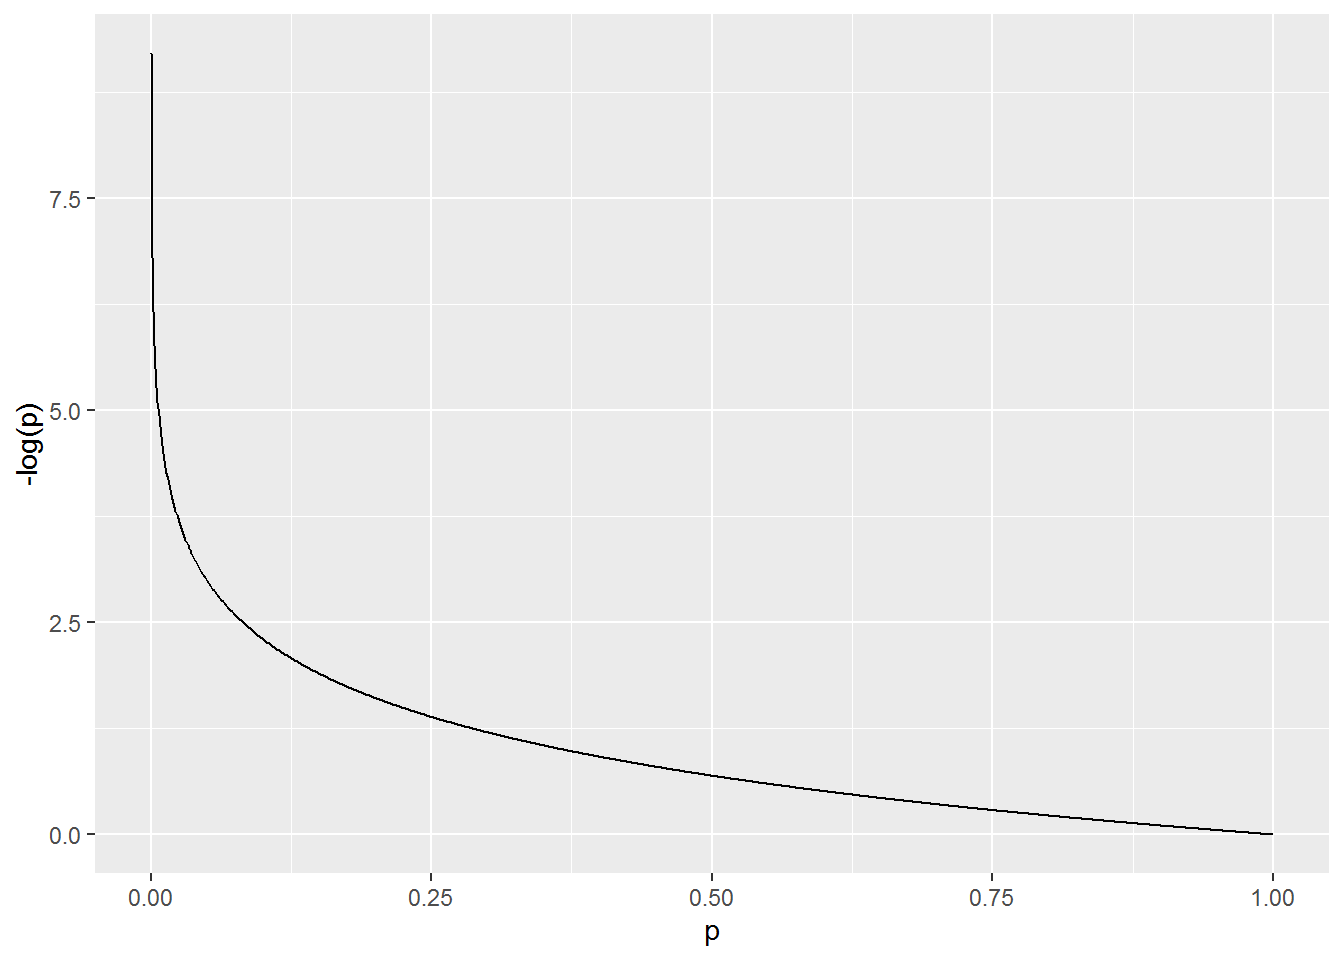
\includegraphics{notes-on-statistical-rethinking_files/figure-latex/unnamed-chunk-24-1.pdf}

The \(2\) is there to facilitate significance testing for \emph{nested} models. Models \(\Theta1\) and \(\Theta2\) are nested, if \(\Theta2\) has all predictors of \(\Theta1\) plus \emph{k} predictors. E.g., model \(Divorce = Marriage~Rate\) is nested inside \(Divorce = Marriage~Rate + Marriage~Age\) with later model having 1 more parameter. Your actual model \(\Theta\) is nested inside the saturated model \(\Theta_s\) that has \(k = n - k_{model}\) more parameters, where \(n\) is sample size and \(k_{model}\) is number of parameters in your model. It turns out that in this case, you can determine whether the difference in goodness-of-fit between two models is significant using chi-squared distribution with \emph{k} degrees of freedom. The only catch is that log-ratio is half the magnitude, so you need that \(2\) to match things up\footnote{I did not follow the derivation of that correspondence yet, so I cannot comment on how and why.}.

At this point, you might remember that the definition of deviance in the book was for a single model:
\[D = -2 \cdot log(p(y|\Theta))\]

Unfortunately, same term can be used both ways, to refer to a log likelihood of a single model or, technically more correctly, to the log-ratio you saw above. In reality, you will mostly see deviance defined as in the book because it is used to compare nested models via chi-square distribution as I've described above, with only difference that you compare any two nested models, not just to a saturated one. This is how nested models are frequently compared, for example, see \href{https://stat.ethz.ch/R-manual/R-patched/library/stats/html/anova.html}{anova()} function in R.

Note that a deviance for a single model still expresses the same idea of goodness-of-fit but is merely not normalized. Thus deviance as in the book \(D = -2 \cdot log(p(y|\Theta))\) corresponds to sum of residuals (absolute values mean nothing but you can use them to compare two models on the same data), whereas \emph{total} deviance corresponds to the \(R^2\) (values are directly interpretable, theoretically, you can use them to compare models fit on different samples).

\hypertarget{general-idea-information-criteria-as-miles-per-gallon}{%
\section{General idea: information criteria as miles-per-gallon}\label{general-idea-information-criteria-as-miles-per-gallon}}

The general formula for all information criteria discussed below is
\[-2\cdot log \left( \frac{goodness~of~fit}{model~complexity} \right)\]

The goodness-of-fit in the numerator is the likelihood, the joint probability of observing the model given each data point \(\prod_i p(\Theta|y_i)\). The denominator expresses model complexity, i.e., its flexibility in fitting the sample and, therefore, its tendency to overfit. Thus, the fraction itself is \emph{goodness-of-fit per unit of model complexity}. This is like miles-per-gallon for car efficiency, so better models are more efficient models, churning out more goodness per complexity.

The numerator is the same for all information criteria discussed below and they differ only in how they compute the model complexity.

\hypertarget{akaike-information-criterion-aic}{%
\section{Akaike Information Criterion (AIC)}\label{akaike-information-criterion-aic}}

The formula most commonly used is
\[ AIC = -2\cdot log(p(\Theta|y)) + 2k \]
where \(k\) is the number of parameters of the model. If you are not a mathematician who is used to translate back-and-forth using logarithms, you may fail spot to the ratio I was talking about earlier. For this, you need to keep in mind that \(log(\frac{a}{b}) = log(a) - log(b)\) and that \(a = log(exp(a))\). Let us re-arrange a bit to get the log-ratio back:
\[ AIC = -2\cdot log(p(\Theta|y)) + 2k \]
\[ AIC = -2 (log(p(\Theta|y)) - k)\]
\[ AIC = -2 (log(p(\Theta|y)) - log(exp(k))\]
\[ AIC = -2 \cdot log \left(\frac{p(\Theta|y)}{exp(k)} \right)\]
And here it is, the log-ratio I've promised! As you can see, AIC assumes that model complexity grows exponentially with the number of parameters. In other words, adding another parameter increases complexity \textasciitilde{}\(2.718\) times.

If you are to use AIC, the current recommendation is to \emph{correct it} with an extra penalty for the size of the sample
\[AICc = AIC + \frac{2k^2 + 2k}{n - k - 1}\]
where \(n\) is the sample size. I won't do it here but you should be able to work out how it is added into the exponent in the denominator.

\hypertarget{bayesian-information-criterion-bic}{%
\section{Bayesian information criterion (BIC)}\label{bayesian-information-criterion-bic}}

A.k.a. Schwarz information criterion (SIC, SBC, SBIC). The motivation is the same as with AIC but the complexity term, in addition to the number of parameters, also reflects the sample size \(n\).

\[BIC = -2\cdot log(p(\Theta|y)) + log(n) k \]

Let us do re-arranging again
\[BIC = -2\cdot log(p(\Theta|y)) + log(n) k \]
\[BIC = -2 \left( log(p(\Theta|y)) + log(n) \frac{k}{2} \right) \]
\[BIC = -2 \left( log(p(\Theta|y)) - log \left(exp(log(n) \cdot \frac{k}{2} \right) \right) \]

For the complexity term, we need to keep in mind that \(exp(a \cdot b) = exp(a)^b\). Thus,
\[exp \left(log(n) \cdot \frac{k}{2} \right)= exp(log(n)) ^ \frac{k}{2} = n^\frac{k}{2}\]
Putting the complexity term back, we get
\[BIC = -2 \left( log(p(\Theta|y)) - log \left(n^\frac{k}{2} \right) \right)\]
\[BIC = -2 \cdot log \left(\frac{p(\Theta|y)}{n^\frac{k}{2}} \right)\]
Thus, we end up with very similar power law complexity term which uses sample size instead of Euler's number as the base.

\hypertarget{problem-of-aic-and-bic-one-size-may-not-fit-all}{%
\section{Problem of AIC and BIC: one size may not fit all}\label{problem-of-aic-and-bic-one-size-may-not-fit-all}}

Both AIC and BIC assume that model complexity and flexibility, that leads to overfitting, is reflected in the number of parameters \emph{k}. However, this is a fairly indirect measure of a model flexibility, based on how models in general tend to overfit data in general. But you probably want to know how your specific model uses its parameters to fit your specific sample and how much overfitting you should expect in that specific case. Because even if a parameter is present in the model, it may not be able to fully use it in case of regularization or multilevel models.

Regularization, in form of strong priors, lasso/ridge regression, etc., restricts the range of values that a given parameter can take. Thus, a model cannot exploit it as much as \emph{other} parameters and will be less able to use it to improve fit to the sample. Similarly, in hierarchical multilevel modeling, you may have dozens or hundreds of parameters that describe intercepts and/or slopes for individual participants (random factors, in general), but most of them could be trivially average (same as or very similar to the group average) and contribute little to the actual fit. In these cases, a simple raw count, which treats all parameters as equals, will overestimate model complexity.

The desire to go beyond one-size-fits-all approach and be as model- and data-specific led to development of deviance information criterion (DIC) and widely-applicable information criterion (WAIC). Both use posterior distribution of \emph{in-sample} deviance and base their penalty on how \emph{variable} this posterior distribution is. Higher variance, meaning that a model produces very different fits ranging from excellent to terrible, hints that model is too flexible for its own good and leads to higher complexity estimate (penalty for overfitting). Conversely, very similar posterior deviance (low variance) means that model is too restricted to fine-tune itself to the sample and its complexity is low.

If you understand why variance of the posterior distribution of divergence is related to models' flexibility and, therefore, to the number of effective parameters, just skip the next section. If not, I came up with a musical instruments metaphor that I and at least some people I've tested it upon found useful.

\hypertarget{musical-instruments-metaphor}{%
\section{Musical instruments metaphor}\label{musical-instruments-metaphor}}

Imagine that you are trying to play a song that you have just heard. But the only instrument you have is a triangle. This is not a particularly flexible instruments pitch-wise, so your rendition of that song will not be very good (your model underfits the data). The good news is that even if you do your worst and do not really try, no one will notice because your worst performance will sound very much like your best one. Simply because it is very hard to make songs sound different using a triangle. Thus, if you play that song many times, trying different versions of it with us judging how close you are to the original, the score we will give you will be very similar (low variance of the deviance for fitting to sample).

But what if I give you an instrument that can vary the pitch at least a bit, like a xylophone for children. Now you more expressive freedom and your version of the music will sound much more like the original. But, it also gives you an opportunity to make a mess of it, so your rendition might sound nothing like the music you've just heard. Thus, the instrument increases the difference between the best and the worst possible performance, so the variance of your performances (on how close they are to the original) also increases (higher variance of the deviance). A more flexible instrument will make the difference even bigger. Think violin or trombone which are not restricted to the scale, so you can play any sound in between and you can match the music you just heard exactly. Imagine that the music your just hear has an odd off-the-scale sounds. Was a defect of the turntable, which cannot go at constant speed, so overall pitch wobbles overtime (noise)? Or is it an experimental music piece designed to sound odd (signal)? If you do not know for sure, you will try to play as close to the original music your heard as possible, matching those off-scale sounds. And, because you can play any sound, your range of possible performance is even larger from one-to-one to ``please, have mercy and stop!'' (even larger variance of deviance).

In short, variance of your performance (posterior divergence) reflects how flexible your instrument is. But why is it indicative of the \emph{effective} number of parameters? Here are regularizing priors in the world of music instrument metaphor. Imagine that in addition to the triangle, I also give you a rubber bell (it was used in a super-secret meeting in Stanislaw Lem's Eleventh Voyage of Ijon Tichy, so that no one would hear when they ring that bell!). Now, technically you have two instruments (your number of parameters is 2) but that bell does not affect your performance (we put very strong regularizing priors so that coefficients are zero or something very-very close to zero). Thus, your ability to play the song did not change and your variance of performance stays the same. Two actual instruments, but only one ``effective'' one. Or, I give you a piano but allow you to use only one octave and only white keys. Yes, you have a piano but with this regularization it is as complex as as kids' xylophone. The \emph{potential} number of notes you can play is great (AIC and BIC would be very impressed and slap a heavy penalty on you) but the actual ``effective'' range is small. Or, you regularize yourself to play scale only notes using violin (something you learn to do). In all of these cases, you deliberately restrict yourself. But why? Why not just play as you heard it (why not fit as well as you can?)? Because if the song you heard is short (sample is small), regularization based on your knowledge about real life helps you to ignore the noise that is always present. E.g., you know that song is for kids' xylophone, so even if you heard notes outside of a single octave that was probably a problem with recording. Or, you never heard that piece for violin but you do know other works of this composer and they always use scale-only notes, so you should not use my violin to play off-scale sounds.

Multilevel models also limit the actual use of parameters. Imagine you heard a recording of a symphonic orchestra. Lots of violins but you figured out that most of them actually play the same melody. So you can get away with using one violin score (sample group average) and assume that most violins play like that (most participants are very close to group average). Any deviations from that group melody are probably mistakes by individual musicians, not the actual melody. Same goes if you hear a choir. Again, many people sing (lots of parameters!) but, mostly, in unison, so you do not need to create an individual score sheet (parameter) for each singer, just one per group of singers.

Wrapping up the metaphor, the more flexible your instrument is, the more variable your performance can be, the easier it is for you to mimic noise and imperfections of the recording that have nothing to do with the piece itself. But when you play it next time, matching the recording with all its noise and distortions perfectly, people who know the piece will be puzzled or may not even recognize it (poor out-of-sample predictions). Adopting the melody for a more limited instrument may make it easier for others to recognize the song! Thus, higher variance in performance accuracy (higher variance of deviance) indicates that you can overfit easily with that instrument (model) and you should be extra careful (impose higher penalty for complexity).

\hypertarget{deviance-information-criterion-dic-and-widely-applicable-information-criterion-waic}{%
\section{Deviance information criterion (DIC) and widely-applicable information criterion (WAIC)}\label{deviance-information-criterion-dic-and-widely-applicable-information-criterion-waic}}

The two are very similar, as both compute the model complexity based on posterior distribution of log likelihood. The key difference is that DIC sums the log likelihood for each model (sample) first and then computes the variance. WAIC computes variance of log likelihood per point and then sums those variances up. In the musical instrument metaphor, for DIC you perform the piece many times (generate many posterior samples), compute accuracy for each performance (deviance for a single sample), and then compute how variable they are. For WAIC, you go note by note (observation by observation). For each note you compute variance over all sample to see how consistent you are in playing it. Then, you sum this up.

\[DIC = -2 \cdot \left( log(p(y|\Theta)) - var(\sum log(p(y|\Theta_i))) \right)\]
\[WAIC = -2 \cdot \left( log(p(y|\Theta)) - \sum_i var(log(p(y_i|\Theta))) \right)\]

The penalty replace \(k\) in AIC and, therefore, will go into the exponent inside the ratio. Again, same idea, that increase in variance of deviance (either per sample in DIC or per point in WAIC) leads to exponentially increasing estimate of complexity.

WAIC is more stable mathematically and is mode widely applicable (that's what statisticians tell us). Moreover, its advantage is that it explicitly recognizes that not all data points in your sample are equal. Some (outliers) are much harder to predict than others. And it is variance of log likelihood for these points that determines how much your model can overfit. An inflexible model will make a poor but consistent job (triangles don't care about pitch!), whereas a complex model can do anything from spot-on to terrible (violins can do anything). In short, you should use WAIC yourself but recognize DIC when you see it and think of it as somewhat less reliable WAIC, which is still better than AIC or BIC when you use regularizing priors and/or hierarchical models.

\hypertarget{importance-sampling}{%
\section{Importance sampling}\label{importance-sampling}}

Importance sampling is mentioned in the chapter but is never explained, so here is a brief description. The core idea is to pretend that you sample from a distribution you need (but have no access to) by sampling from another distribution (the one you have access to) and ``translating'' the probabilities via \emph{importance ratios}. What does this mean?

Imagine that you want to know an average total score for a given die after you throw it ten times. The procedure is as simple as it gets: you toss the die ten times, record the number you get on each throw, sum them up at the end. Repeat the same toss-ten-times-and-sum-it-up as many times as you want and compute your average. But what if you do not have access to that die because it is \emph{the die} and is kept under lock in International Bureau of Weights and Measures? Well, you have \emph{a die} which you can toss and you have a list of \emph{importance ratios} for each number. These \emph{important ratios} tell you how much more likely is the number of \emph{the die} (the one you are after) compared to \emph{a die} you have in your hand. Let's say the importance ratio for \emph{1} (so, number 1 comes up on top) is \texttt{3.0}. This means that whenever \emph{your die} gives you \emph{1}, you assume that \emph{the die} came up \emph{1} on \textbf{three} throws. If the importance ratio for \emph{2} is 0.5, whenever you see \emph{2} on your die, you record only half the throw (\emph{2} comes up twice as rarely for real die than for your die, so two throws that give you \emph{2} amount to a single throw). This way you can toss your die and every toss equates to different number of throws that generated the same number for \emph{the die}. So, you sample your die but record outcomes for the other die. Funny thing is that you don't even need to know how fair your die is and what is the probability of individual sides. As long as you know the importance ratios, keep tossing it and translating the probabilities, you will get the samples for the die you are interested in.

Note that if you toss your die ten times, the translated number of tosses for \emph{the die} does not need to add up to ten. Imagine that, just by chance, you got \emph{1} four times. Given the importance ratio of \texttt{3.0} that alone translates into twelve tosses. Solution? You \emph{normalize} your result by \emph{sum of importance ratios} and get back you ten tosses.

The very obvious catch is, \emph{how do we know the importance ratios}? Well, that is situation specific. Sometimes, we can compute them because we know both distributions, it just that one is easier to sample than the target one (so, we optimize the use of computing power). Sometimes, as in case of PSIS/LOO below, we can use an approximation.

\hypertarget{pareto-smoothed-importance-sampling-leave-one-out-cross-validation-psisloo}{%
\section{Pareto-smoothed importance sampling / leave-one-out cross-validation (PSIS/LOO)}\label{pareto-smoothed-importance-sampling-leave-one-out-cross-validation-psisloo}}

The importance sampling I've described above is the key to the PSIS/LOO. The idea is the same, we want to sample from the posterior of the model that was fitted \emph{without} a specific data point \(y_i\) (we write it as \(p(\Theta_{-i,s}|y_i)\)). But we do not really want to refit the model. Instead, we want to use what we already have, samples from the model that was fit on all the data, \emph{including} point \(y_i\). So, we pull of the same importance sampling trick, sampling from \(p(\Theta_s|y_i)\) and translating it to \(p(\Theta_{-i,s}|y_i)\). The only thing we need are importance factors\footnote{Unfortunately, I did not yet follow the derivation of this proportionality, so I cannot explain why this is the case mathematically.}
\[r_i = \frac{p(\Theta_{-i,s}|y_i)}{p(\Theta_s|y_i)} \propto \frac{1}{p(y_i|\Theta_s)}\]

The importance ratio tells you that decrease in your ability to predict an observation out-of-sample is proportional to difficulty of predicting in-sample. Here is an intuition behind this. \emph{Any} observation will be harder to predict, if it was not included into the data the model was trained on. This is because, in its absence the model will use its parameters to fit the data that is present, including fitting noise, if it has spare parameters. So, you expect that out-of-sample deviance (\(p(y_i|\Theta_{-i}\)) should be always worse than in-sample deviance for the same observation (\(p(y_i|\Theta\)). How much worse depends on how ``typical'' the observation is. If it is typical and ``easy'' for a model to predict, in its absence the model will still see many similar ``typical'' observations and will be well prepared to predict it. However, if the observations is atypical, an outlier, the model won't see too many observations that are alike and will concentrate more on typical points.

I.e., assume that out-of-sample deviance is in-sample deviance squared (the importance ratio we use goes in that direction). Asume that our \emph{in-sample} deviance is 60, 40, and 50 in one case and 10, 10 and 130 in the other case. Both deviances sum up to 150, so from \emph{in-sample} point of view they are equal. However, approximating \emph{out-of-sample} deviance as a square of \emph{in-sample} deviance makes for a dramatic difference. For the first case, it jumps to 7700 but the second case to 17100, more than twice the difference. This is because in second case \emph{out-of-sample} deviance is dominanted by that single very difficult point, which will be terribly difficult out-of-sample.

This explosive powerlaw-like scaling of expected out-of-sample deviance is the reason for warnings that LOO/PSIS generates. A single very difficult observation can be single-handedly responsible for most of the deviance, making it hard to understand whether the model is good or bad on the rest of observations. Thus, you should consider what this extreme outlier means for your understanding of the process. Is it so different because it was recorded wrongly (the responsible person pressed 1 instead of 7)? Is this an extreme response time because a participant was distracted on that trial and started paying attention to the task only 15 seconds after the trial began? Is it an important observations that indicates that you are ignoring a really important predictor? You should think carefully about it and decide on whether you treat that observation differently (e.g., allowing for larger uncertainty for that point because you think this is mostly noise) or you change your model to better account for it.

\hypertarget{bayes-factor}{%
\section{Bayes Factor}\label{bayes-factor}}

Not an information criterion. However, it is a popular way to compare Bayesian models. Compared to information criteria, the logic is reversed. In case of the information criteria, we are asking which \textbf{model fits data} the best given the penalty we impose for its complexity. In case of Bayes Factor, we already have two models (could be different models with different number of parameters or just with different parameter values) and we are interested how well the \textbf{data matches models} we already have.

Let's start with the Bayes theorem:
\[Pr(M|D)=\frac {\Pr(D|M)\Pr(M)}{\Pr(D)}\]
where, \emph{D} is data and \emph{M} is the model (hypothesis). The tricky part is the marginal probability (prior) of data \(Pr(D)\). We hardly ever know it for sure, making computing the ``correct'' value for \(Pr(M|D)\) problematic. When using posterior sampling, we side-step the issue by ignoring it and normalizing the posterior by the sum of the posterior distribution. Alternatively, when comparing two models, you can compute their ratio:
\[{\frac {\Pr(D|M_{1})}{\Pr(D|M_{2})}}={\frac {\Pr(M_{1}|D)}{\Pr(M_{2}|D)}} \cdot {\frac {\Pr(M_{1})}{\Pr(M_{2})}}\]
here \(\frac{\Pr(D|M_{1})}{\Pr(D|M_{2})}\) are \textbf{posterior odds}, \(\frac {\Pr(M_{1}|D)}{\Pr(M_{2}|D)}\) is \textbf{Bayes Factor}, and \(\frac {\Pr(M_{2})}{\Pr(M_{1})}\) are \textbf{prior odds}. The common \(Pr(D)\) nicely cancels out!

If you assume that both hypotheses/models are equally likely (you have flat priors), the prior odds are 1:1 and your posterior odds are equal to Bayes Factor or, vice versa, Bayes Factor is equal to posterior odds. This means you can just pick their likelihoods from the posterior sampled distribution and compute the ratio.

I am not a big fan of Bayes Factor for conceptual reasons. Although it can compare any two models (as long as the sample is the same), it looks a lot like a Bayesian version of a p-value and, therefore, lends itself naturally to the null-hypothesis testing. And, as far as my reading of literature in my field is concerned, this is how people most frequently use it, as a cooler Bayesian way of null-hypothesis testing. You have no worries about multiple comparisons (it is Bayesian, so no need for error correction!) and it can prove null hypothesis (it is the ratio, so flip it and see how much stronger \emph{H0} is)! There is nothing wrong with this per se but the advantage of Bayesian statistics and information criteria is that you do not \emph{need} to think in terms of null hypothesis testing and nested models. Adopting Bayes Factor may prevent you from seeing this and will allow you to continue doing same analysis just in a differently colored wrapper. Again, there is nothing wrong with exploratory analysis using null hypothesis testing until you can formulate a better model. But it should not be the \emph{only} way you approach modeling.

\hypertarget{bayesian-versus-frequentist-statistics}{%
\chapter{Bayesian versus Frequentist Statistics}\label{bayesian-versus-frequentist-statistics}}

I suspect that many student who read ``Statistical Rethinking'' have a feeling that it is something completely different from what they have been learning in ``traditional'' statistics classes. That Bayesian approach is more ``hands-on'' and complicated, whereas ``normal'' statistics is simpler and easy to work with even it is ``less powerful.''\footnote{Not really.} Thus, the purpose of this note is to walk you through a typical statistical analysis and focus on practical differences and, more importantly, similarity of the two approaches.

\hypertarget{choice-of-likelihood-both}{%
\section{Choice of likelihood (both)}\label{choice-of-likelihood-both}}

The very first we do is to look at the data and decide which distribution we will use to model the data / residuals be it normal, binomial, Poisson, beta, etc. That is the very first line of our models that goes like this
\[
\color{red}{y_i \sim Normal(\mu_i, \sigma)} \\
\mu_i = \alpha + \beta_{x1} \cdot X1 + \beta_{x2} \cdot X2 + \beta_{x1\cdot x2} \cdot X1 \cdot X2 \dotso \\
\alpha \sim Normal(0, 1) \\
\beta_{x1} \sim Exponential(1) \\
\cdots \\
\sigma \sim Exponential(1)
\]

This decision is neither Bayesian, nor frequentist. This is a decision about the model that best describes the data, so it is independent of the inference method you will use. This is a decision that you are making even if you are using ``prepackaged'' statistical tests like the t-test or ANOVA that assume normally distributed residuals\footnote{Admittedly, in this case people often start with the statistical test and see whether data is suitable rather than the other way around.}.

\hypertarget{linear-model-both}{%
\section{Linear model (both)}\label{linear-model-both}}

Next, you decide on the deterministic part of the model that expresses how a parameter of the distribution you chose on the previous step is computed from various predictors. E.g., for the linear regression with normally distributed residuals, you decide which predictors do you use to compute the mean. The model line would look something like this
\[
y_i \sim Normal(\mu_i, \sigma) \\
\color{red}{\mu_i = \alpha + \beta_{x1} \cdot X1 + \beta_{x2} \cdot X2 + \beta_{x1\cdot x2} \cdot X1 \cdot X2 \dotso} \\
\alpha \sim Normal(0, 1) \\
\beta_{x1} \sim Exponential(1) \\
\cdots
\]
Again, this is neither Bayesian, nor frequentist decision, it is a linear model decision. Chapters 4-6 and 8 concentrate on how to make this decision using directed-acyclic graphs (DAGs) and introduce concepts of multicollinearity, colliders and bias they can produce, backdoor paths and how to identify them, etc. They explain how you can make educated decision on which predictors to use based on your knowledge of the field or of the problem. At this stage you also decide on whether to normalize data, as it could make interpreting the model easier.

You always have to make this decision. For example, if you use the (repeated measures) ANOVA, you do need to decide which factors to use, whether to include interactions, should you transform the data to make coefficients directly interpretable, do you use a link function, etc.\footnote{However, you do see cases when one simply throws all factors and interactions into the pot with little regard for an underlying causal model or interpretability of the coefficients.}

\hypertarget{priors-optional-for-bayesian}{%
\section{Priors (optional for Bayesian)}\label{priors-optional-for-bayesian}}

Priors are a Bayesian way to regularize the model, so this is something you do need to think about when doing Bayesian statistics\footnote{Modern packages like \emph{brms} make it easy for you by deducing a set of reasonable priors for you. However, it is always a good idea to double-check them.}. In a model this part would look something like this
\[
y_i \sim Normal(\mu_i, \sigma) \\
\mu_i = \alpha + \beta_{x1} \cdot X1 + \beta_{x2} \cdot X2 + \beta_{x1\cdot x2} \cdot X1 \cdot X2 \dotso \\
\color{red}{\alpha \sim Normal(0, 1) \\
\beta_{x1} \sim Exponential(1) \\
\cdots}
\]

This is probably a decision that students worry about the most as it feels more subjective and arbitrary than other decisions, such as choice of the likelihood or predictors. Chapter 4 through 7 gave you multiple examples that there is nothing particularly arbitrary about these choices and that you can come up with a set of justifiable priors based on what you know about the topic or based on how your pre-processed the data\footnote{In my experience, people tend to worry about priors for data unseen. Some kind of data of which you know absolutely nothing, hence, have trouble deducing priors. In practice, you always know something about the topic and the data. If not, you should read on it instead of using flat priors!}.

Still, I think for a lot of people ``normal'' statistics with its flat priors feels simpler and also more objective and, therefore, more trustworthy (``we did not favor any specific range of values!''). If that is the case then use flat priors (but see the side note below) making Bayesian and frequentists models identical! For me, though, writing it down explicitly makes one realize that range \(-\infty, +\infty\) is remarkably large to the point of being an obvious overkill
\[
y_i \sim Normal(\mu_i, \sigma) \\
\mu_i = \alpha + \beta_{x1} \cdot X1 + \beta_{x2} \cdot X2 + \beta_{x1\cdot x2} \cdot X1 \cdot X2 \dotso \\
\color{red}{\alpha \sim Uniform(-\infty, +\infty) \\
\beta_{x1} \sim Uniform(-\infty, +\infty) \\
\cdots}
\]

In short, Bayesian inference gives you an \emph{option} to specify priors. You do not need to take on the option and can use flat frequentist's priors.

\emph{Side note.} In reality, flat priors are never good priors. If there is sufficient data then, in most cases, the priors (flat or not) do not have much influence. However, if the data is limited then flat priors almost inevitably lead to overfitting as there is no additional information to counteract the effect of noise. This overfitting may feel more ``objective'' and ``data-driven'' than a more conservative underfitting of data via strongly regularizing priors but the latter is more likely to lead to better out-of-sample predictions and, therefore, are more likely to be replicated.

\hypertarget{maximum-likelihood-estimate-both}{%
\section{Maximum-likelihood estimate (both)}\label{maximum-likelihood-estimate-both}}

Once you fitted the model, you get estimates for each parameter you specified. If you opted for flat priors, these estimates will be the same but for very minor differences due to sampling in Bayesian statistics. If you did specify regularizing priors then estimates will be different, although the magnitude of that difference will depend the amount of data: the more data you have, the smaller the influence of the priors, we closer the estimates will be (see also the side note above). Importantly, both types of inferences will produce (very similar) estimates and you interpret them the same way.

\hypertarget{uncertainty-about-estimates-different-but-comparable}{%
\section{Uncertainty about estimates (different but comparable)}\label{uncertainty-about-estimates-different-but-comparable}}

This is the point where the two approach fundamentally diverge. In case of frenquetists statistics you obtain confidence intervals and p-values based on appropriate statistics and degrees of freedom, whereas in case of Bayesian inference you obtain credible/compatibility intervals and can use posterior distribution for individual parameters to compute probability that they are strictly positive, negative, concentrated within a certain region around zero, etc.

These measures are conceptually different but tend to be interpreted similarly and mostly from Bayesian perspective. I think it is a good idea to compute and report all of them. Typically, they would be close, making you more certain about the results. More importantly, whenever they diverge it serves as a warning to investigate the case and what can cause this difference.

\hypertarget{model-comparison-via-information-criteria-both}{%
\section{Model comparison via information criteria (both)}\label{model-comparison-via-information-criteria-both}}

Both approaches use information criteria to compare models with Akaike and Bayesian/Schwarz information criteria being developed specifically for the case of flat priors of frenquetist models. Here, Bayesian approach holds an advantage as the full posterior allows for more elaborate information criteria such as DIC, WAIC, or LOO. Still the core idea and the interpretation of the comparison results are the same.

\hypertarget{generating-predictions-both}{%
\section{Generating predictions (both)}\label{generating-predictions-both}}

You generate predictions using the model definition which is the same for both approach. Hence, you are going to get same predictions, at least for the mean. As the two approach differ in how they characterize uncertainty, the uncertainty of predictions will be different but, typically, comparable.

\hypertarget{conclusions}{%
\section{Conclusions}\label{conclusions}}

As you can see, from \emph{practical} point of view, apart from optional Bayesian priors and different ways to quantify the uncertainty of estimates, the two approaches are the same. They require you making same decisions and the results are interpreted the same way. This lack of difference becomes even more apparent when you use software packages for running your statistical models. E.g., the way you specify your model in \texttt{lme4} (frenquetist) and \texttt{brms} (Bayesian) is very much the same to the point that in most cases you only need to change the function name (\texttt{lmer} to \texttt{brm} or vice versa) and leave the rest the same.

Thus, the point is that you should not be choosing between studying or doing frenquetists or Bayesian statistic. I feel more comfortable with Bayesian, mostly because it makes it easier interpret statistical significance. However, my typical approach is to start with frenquetist statistics (fast, good for shooting from a hip), once I am certain about my decisions (likelihood, model) I re-impliement the same model in Bayesian using informative priors and see whether results match (with reason). Then, I report both sets of inferences. This costs me remarkably little time precisely because there is so little difference between the two approaches from practical point of view!

\hypertarget{take-home-message-1}{%
\section{Take home message}\label{take-home-message-1}}

We are not studying something completely different! We are merely approaching it from an unusual angle that leads to deeper understanding and interesting insights in the long run.

  \bibliography{book.bib}

\end{document}
